\chapter{Power and Reset}

\section{Circuit description}

The figure \ref{fig:artemisa-schematic-power} shows the schematic diagram of the power management and power-on reset circuits.

\begin{figure}[htbp]
  \centering
  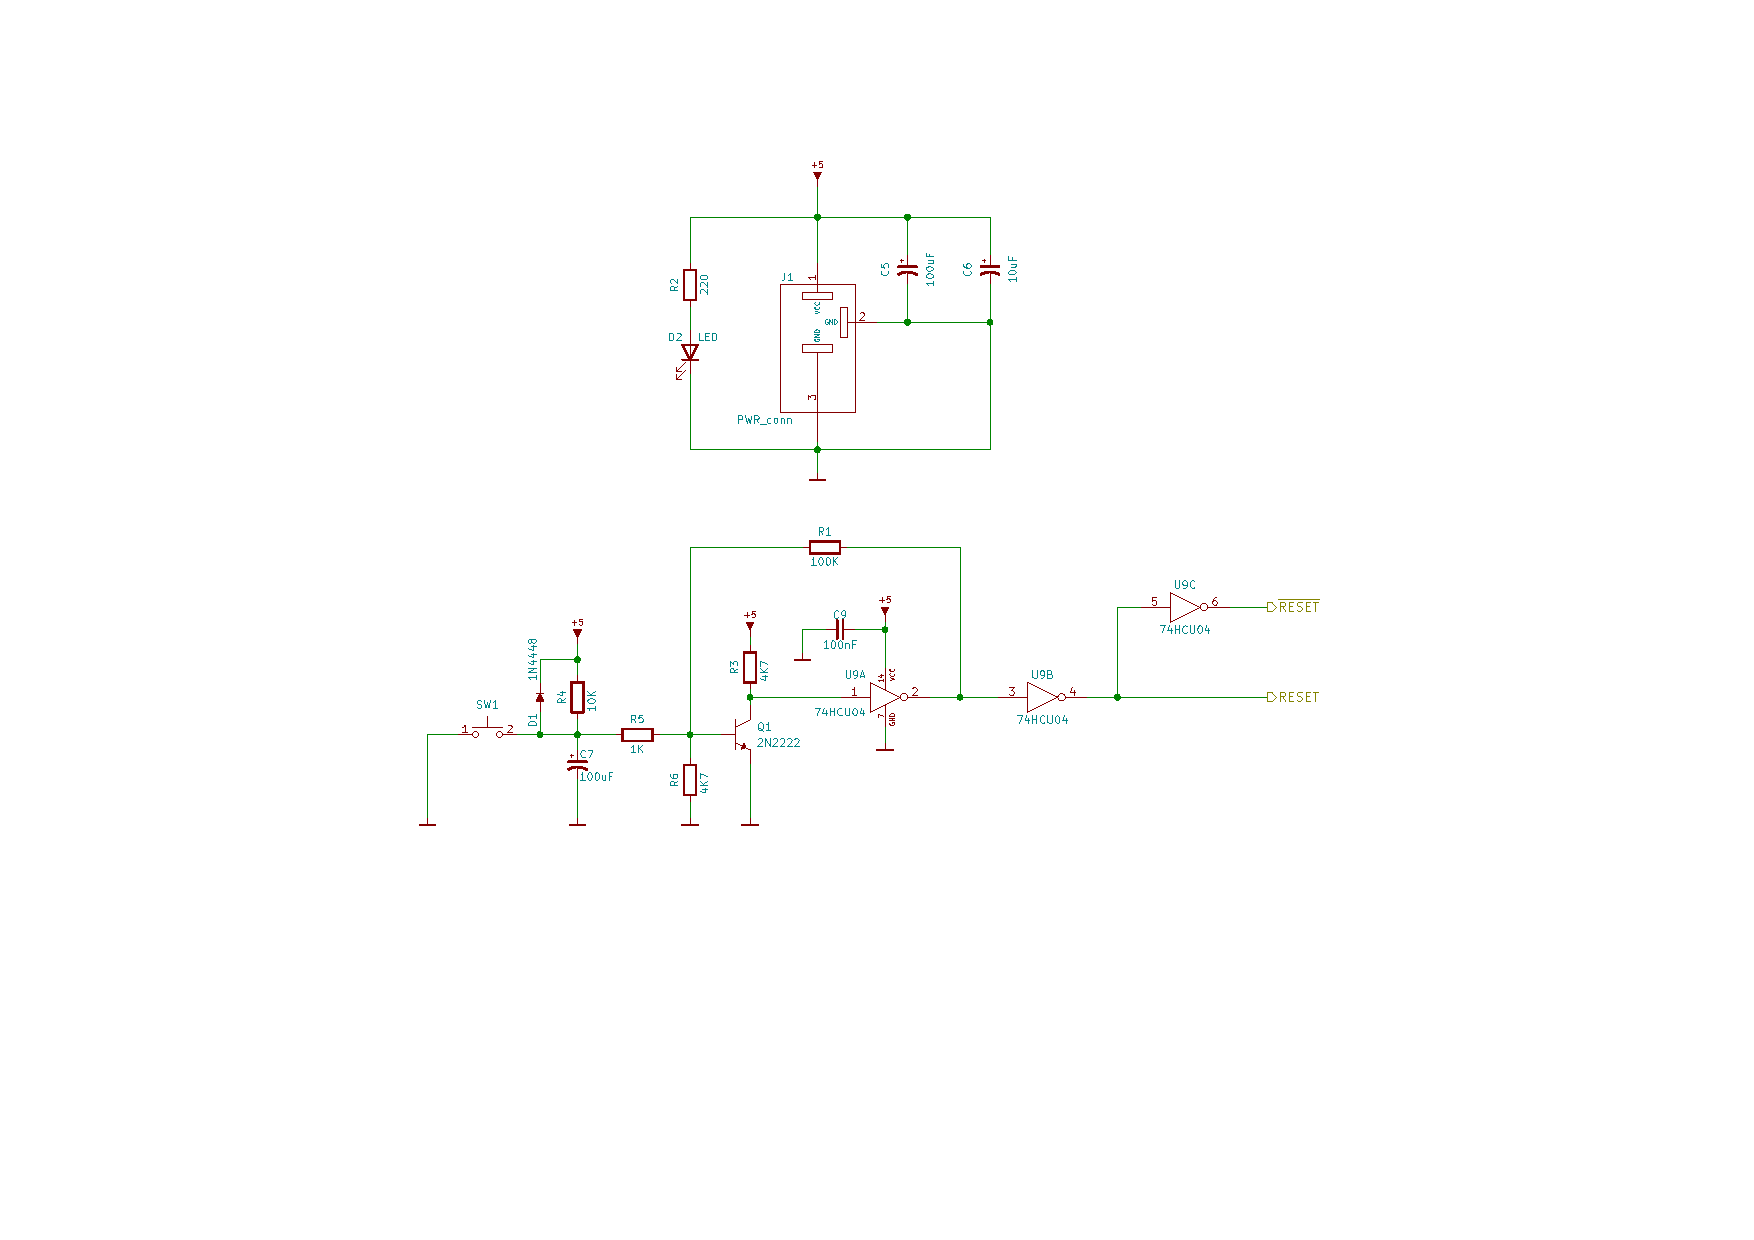
\includegraphics[width=\linewidth,trim={6cm 7cm 6cm 2.5cm},clip]{figures/artemisa-schematic-power}
  \caption{Schematic diagram of power input and power-on reset}
  \label{fig:artemisa-schematic-power}
\end{figure}

As you can see, the schematic sheet is divided in two separated blocks.

\begin{itemize}
  \item At the top side of the schematic we have the power connector circuit. This shows the circuit formed by the DC power barrel connector and a few auxiliary elements around it.
  \item At the bottom side of the schematic we have the power-on reset circuit. This contains the reset button and several components aimed to generate a reset signal to get several computer devices to their initial state.
\end{itemize}

We will analyze each subcircuit separately.

\subsection{Power connection}

Starting with the power connector. This is extremely simple, as shown in \ref{fig:artemisa-schematic-power-conn}. The DC barrel connector {\tt J1} provides three different terminals: 1, 2 and 3. 1 is the positive input terminal, or {\tt VCC}. 2 and 3 are the negative input terminals, or {\tt GND}. As you can see, they are directly connected to the {\tt +5} and {\tt GND} power symbols, respectively. This means the DC barrel connector is feeding the five volts and the ground inputs. Whenever we see the {\tt +5} and {\tt GND} power symbols in the schematic, we know they are wired to and powered from the {\tt J1} connector.

\begin{figure}[htbp]
  \centering
  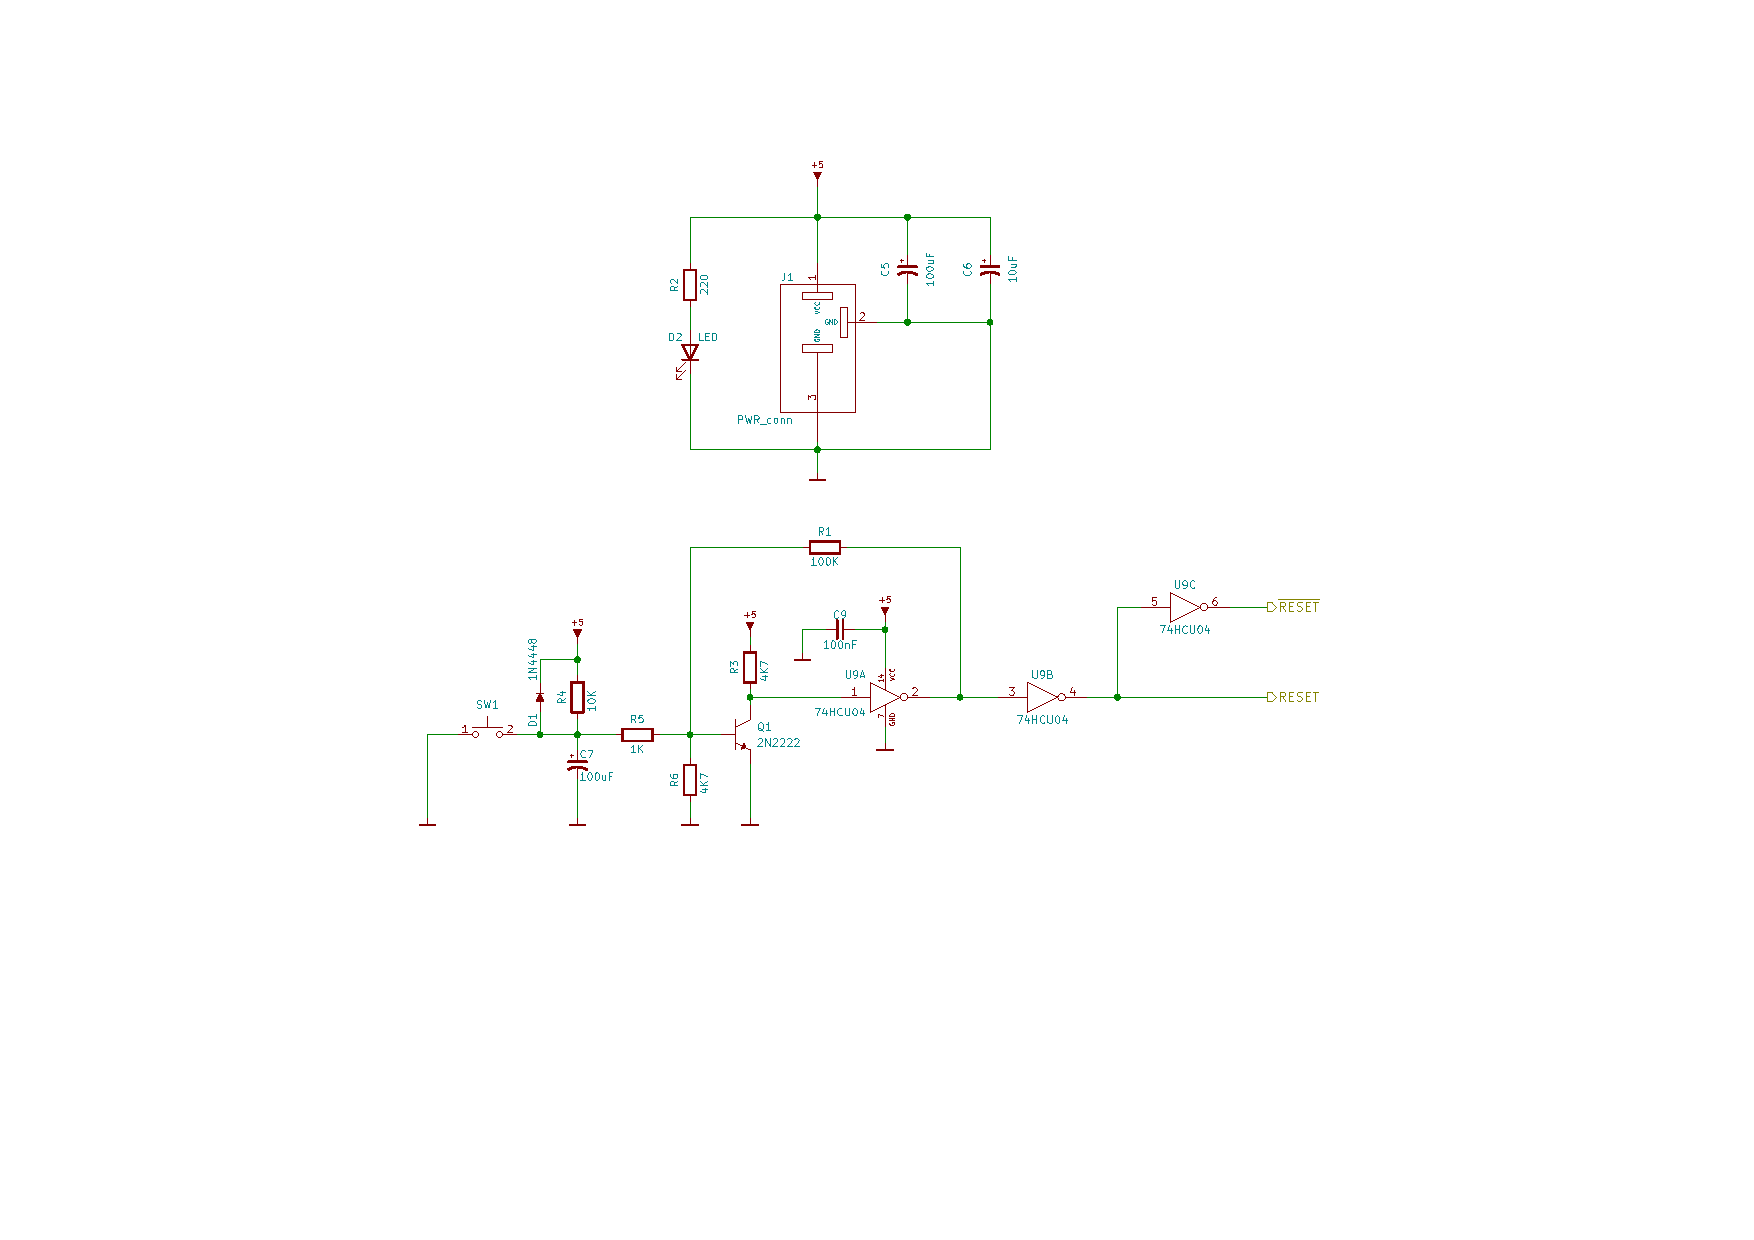
\includegraphics[width=0.5\linewidth,trim={11cm 12.8cm 12.4cm 2.5cm},clip]{figures/artemisa-schematic-power}
  \caption{Schematic diagram of power connector}
  \label{fig:artemisa-schematic-power-conn}
\end{figure}

The LED \toref{diode} {\tt D2} is used to indicate the computer is powered on when the power cable is connected to {\tt J1}. The resistor {\tt R2} is used to limit the current passing throught {\tt D2}.

\begin{theory}[htbp]{Diodes}
  Diodes are semiconductor devices that conduct the electric current only in one direction. They have two terminals: the anode and the cathode. The current flows from the anode to the cathode (forward current), but never from the cathode to the anode (reverse current). The forward current experiments a voltage drop of a few volts caused by the junction of semiconductor material in the diode, typically of 0.6-0.7 volts.\\\\

  LEDs, or light-emitting diodes, are a special kind of diodes that emits light when forward current flows through it. Their voltage drop depends on the color of the light they emit, and it is typically of a few volts. Apart from this particularity, their behavior is the same as any other type of diode.\\\\

  Any diode, LEDs included, does not offer any resistance to the forward current. The current experiments a voltage drop as discussed above. But once that voltage drop is exceeded, all the current will flow following the Ohms law. This means that, in the absence of any other kind of resistor in the circuit, the current will be theorically infinite (as $I = \frac{V}{R}\), when $R\) is zero). Or, in other words, a short-circuit will happen.\\\\

  For that reason, LEDs are always put in series with a resistor that will limit the current that traverses the circuit. Otherwise, we will have a short-circuit that will destroy the LED, and could damage the power supply.
\end{theory}

You can also find two large electrolytic capacitors: {\tt C5} and {\tt C6}. They are \toref{decoupling capacitors} used to filter the voltage fluctuations that may occur in the power adapter connected to {\tt J1}.

\begin{theory}[htbp]{Decoupling capacitors}
  Integrated circuits do not consume an even electric current. They experiment fluctuations. They work like a building. If many occupiers open their water taps, the whole building will demand a high flow of water from the external water supply. If most of them close their taps, the flow will be low. Integrated circuits are made of transistors. And each transistor is equivalent to a water tap. They are open or closed depending on their inputs and their previous states.\\\\

  When part of the circuit experiments a spike in their current demand, the power supply must satisfy it. However, power supplies are not ideal. They will try to adequate the supplied voltage to the new demands. But it does not happen immediately. As result, some parts of the circuit could experiment a brief voltage drop. This can have effects to the integrated circuits, generating errors like misinterpreting digital input values.\\\\

  The way to prevent this is to use decoupling capacitors. They will act as local batteries connected to some part of the circuit. If there is any voltage drop in the power input, the charge of the capacitor will compensate the lost. The capacitor will operate as a power supply for a short period of time (while it is charged), ensuring the voltage level is even regardless the fluctuations in the supply and the demand. In the building analogy, this is like putting a water tank at the input pipe of the building. All occupiers can open their taps all at once. The tank will feed the taps while the water supplier adapts the flow to the new demand.\\\\

  Typically, every integrated circuit has its own small decoupling capacitor to protect it from the voltage fluctuations. There are also some bulk capacitors aimed to decouple the whole power circuit of the board from the power line coming from the DC barrel connector.
\end{theory}

\subsection{Power-On Reset}

The second part of the schematic sheet shown in figure \ref{fig:artemisa-schematic-por} is the power-on reset circuit. This part is by far more complex than the power connector part. And also more complex than most of the circuits we will analyze in this book. So we will explain how it works with an analysis of how the current flows on power on and how it affects the \sym{RESET} and \sym{/RESET} outputs.

\begin{figure}[htbp]
  \centering
  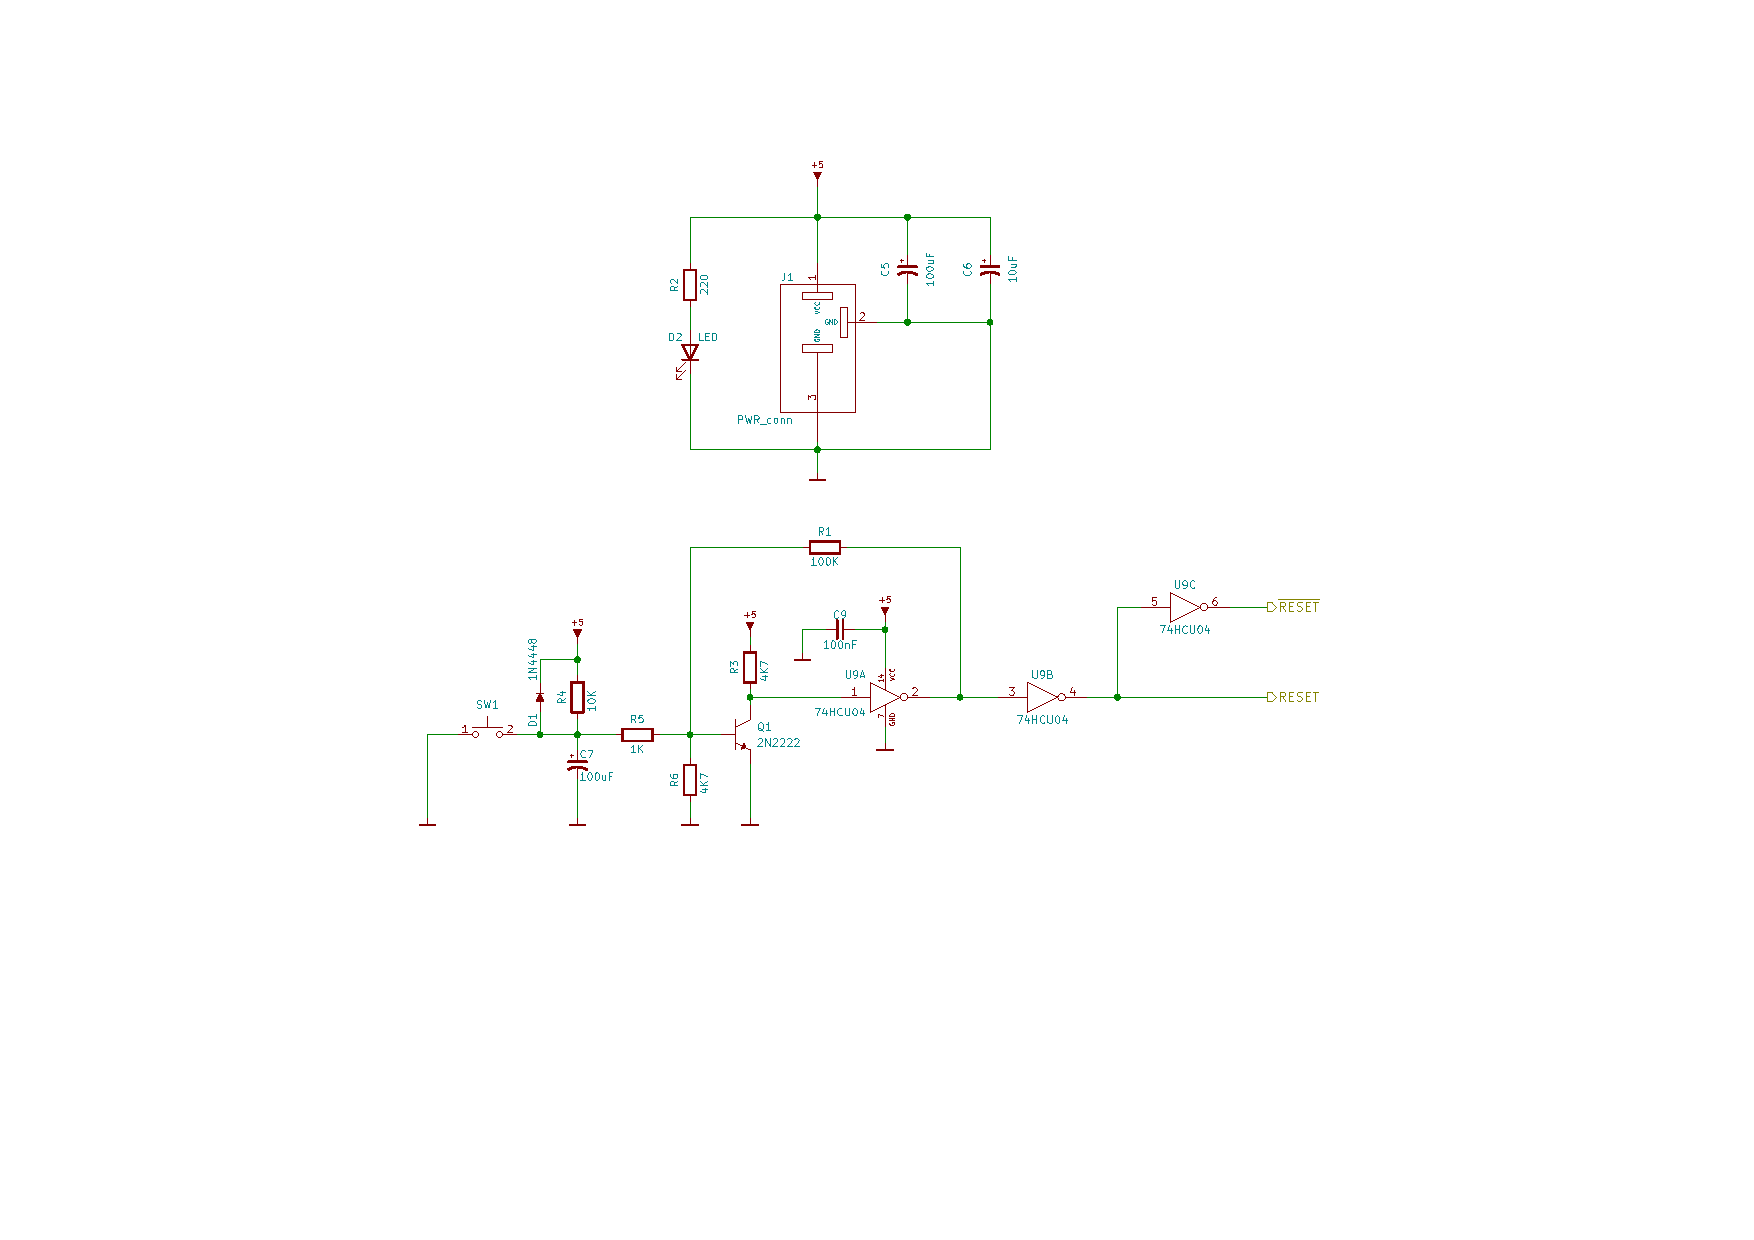
\includegraphics[width=\linewidth,trim={6cm 7cm 6cm 8.5cm},clip]{figures/artemisa-schematic-power}
  \caption{Schematic diagram of power-on reset circuit}
  \label{fig:artemisa-schematic-por}
\end{figure}

We will start assuming we just have connected the power cable to the DC barrel connector. This situation is represented by the simulation shown in Figure \ref{fig:simul-por-01}.

\begin{figure}[htb]
  \centering
  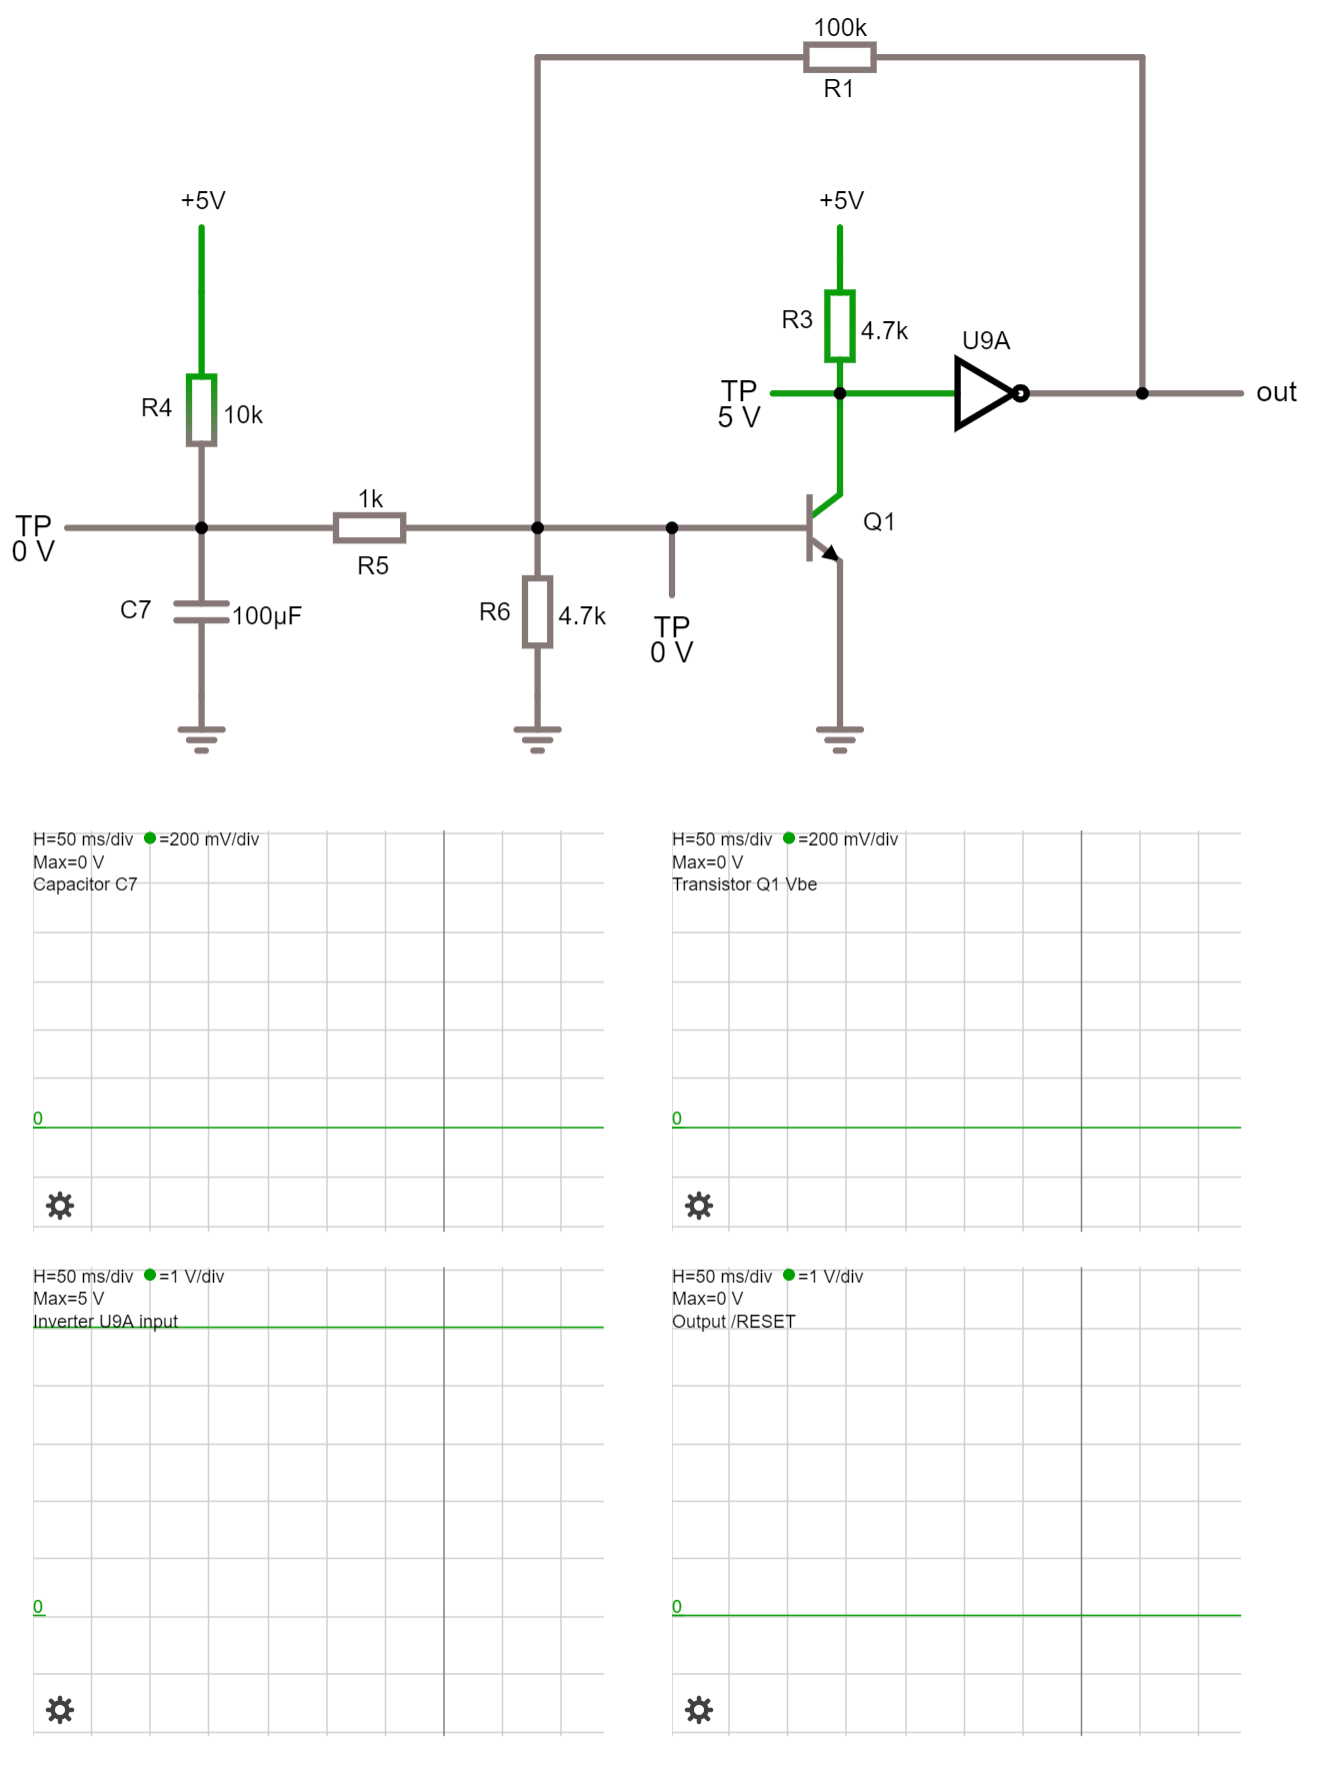
\includegraphics[width=0.7\linewidth]{figures/simul-por-01}
  \caption{Simulation of Power-On Reset: initial state after power on}
  \label{fig:simul-por-01}
\end{figure}

In that instant, the current is ready to flow from the {\tt +5} power supply throught {\tt R4} to reach the positive terminal of the capacitor {\tt C7}. We will assume this capacitor is discharged because the circuit was not energized yet. So the voltage in its positive terminal is initially zero.

As the voltage in {\tt C7} is almost zero, there is almost no current flowing through {\tt R5} or {\tt R6} to the base terminal of \toref{transistor} {\tt Q1}. Thus, the transistor will operate in the cut-off region.

As the transistor is cut-off, its collector-emitter junction is equivalent to an open circuit without any current flowing through the collector terminal. Thus, the 5 volts across {\tt R3} are \toref{transmitted to the input terminal} of the 74HCU04 logic inverter {\tt U9A}. These 5 volts are represented in the simulation circuits like Figure \ref{fig:simul-por-01} with green coloured wires that are turned into grey as their voltage drops to zero.

\begin{theory}[htbp]{Transistors}
  Transistors are semiconductor devices used to amplify or switch electronic signals. They have three terminals. The voltage level between a pair of these terminals determine the current through another pair of terminals. The power of the controlled output can be higher than the power of the controller input. Thus, they can amplify a electric signal.\\\\

  In this particular example of figure \ref{fig:artemisa-schematic-por}, we are using a NPN bipolar transistor for switching purposes. These transistors have three terminals known as base (left), emitter (below, with an arrow) and collector (above). The current between base and emitter ($I_B$) determines the current that will go from the collector to the emitter ($I_C$).\\\\

  \begin{itemize}
    \item When the voltage at the base terminal is low, there will be no current from the base to the emitter. Thus, the transistor will be cut-off and no current will flow. The collector-emitter junction will be equivalent to an open circuit.
    \item If the voltage at the base terminal is high, the transistor will saturate and will let pass as much current as possible from the collector to the emitter. The collector-emitter junction will be equivalent to a closed circuit.
  \end{itemize}
\end{theory}

\begin{theory}[htbp]{Voltage drop when current is zero}
  Perhaps you might wonder why the input terminal of {\tt U9A} has 5 volts when {\tt Q1} is cut-off considering there is a resistor {\tt R3} in the path. The aswer to this is given by the Ohms law.\\\\

  As {\tt Q1} is cut-off, there is only one possible path for the current: from {\tt 5+} to the input terminal of the logic inverter {\tt U9A}. The logic inverter, as any other logic gate, has a huge input impedance around 6M\si{\ohm}. This means the current going through the logic gate input terminal is almost zero. The voltage in the input terminal of {\tt U9A} is the five volts from the power supply minus the voltage drop in {\tt R3}, or $V_{in} = 5v - V_{R3}$. If there is no current, the Ohms law $V=I \cdot R$ reveals the voltage drop $V_{R3}$ is zero. Thus, the voltage at the input terminal of the logic gate is 5 volts.\\\\

  The rule of thumb is that, in the absence of current due to very high impedances, the voltage remains constant in all those points where current is not flowing. No matter the resistors we put on its way.
\end{theory}

As the logic inverter {\tt U9A} receives 5v in its input, or a high level in the digital world, it generates 0v in the output, a low level. That is the out point shown in Figure \ref{fig:simul-por-01}. We could be considered our active-low reset signal. However, it is a good idea to isolate this part of the circuit from the rest of devices that will use the output.

This isolation is done by using {\tt U9B} and {\tt U9C} as buffers. The logic gate {\tt U9B} shown in Figure \ref{fig:artemisa-schematic-por} inverts the output from {\tt U9A}  again, producing a signal labeled as {\tt RESET} whose logic value is high at this instant. {\tt U9C} inverts that signal one more time to generate {\tt /RESET}, the active-low reset signal, which will be low at this point in time.

After this analysis, we can be sure the reset pulse will initiate upon power adapter is plugged into the DC barrel connector. This is represented in the graphs and test points shown in Figure \ref{fig:simul-por-01}. After that instant zero, some milliseconds will pass while the current from the power supply is flowing through {\tt R4} to the input terminal of the capacitor. This is represented by the simulation shown in Figure \ref{fig:simul-por-02}.

\begin{figure}[htb]
  \centering
  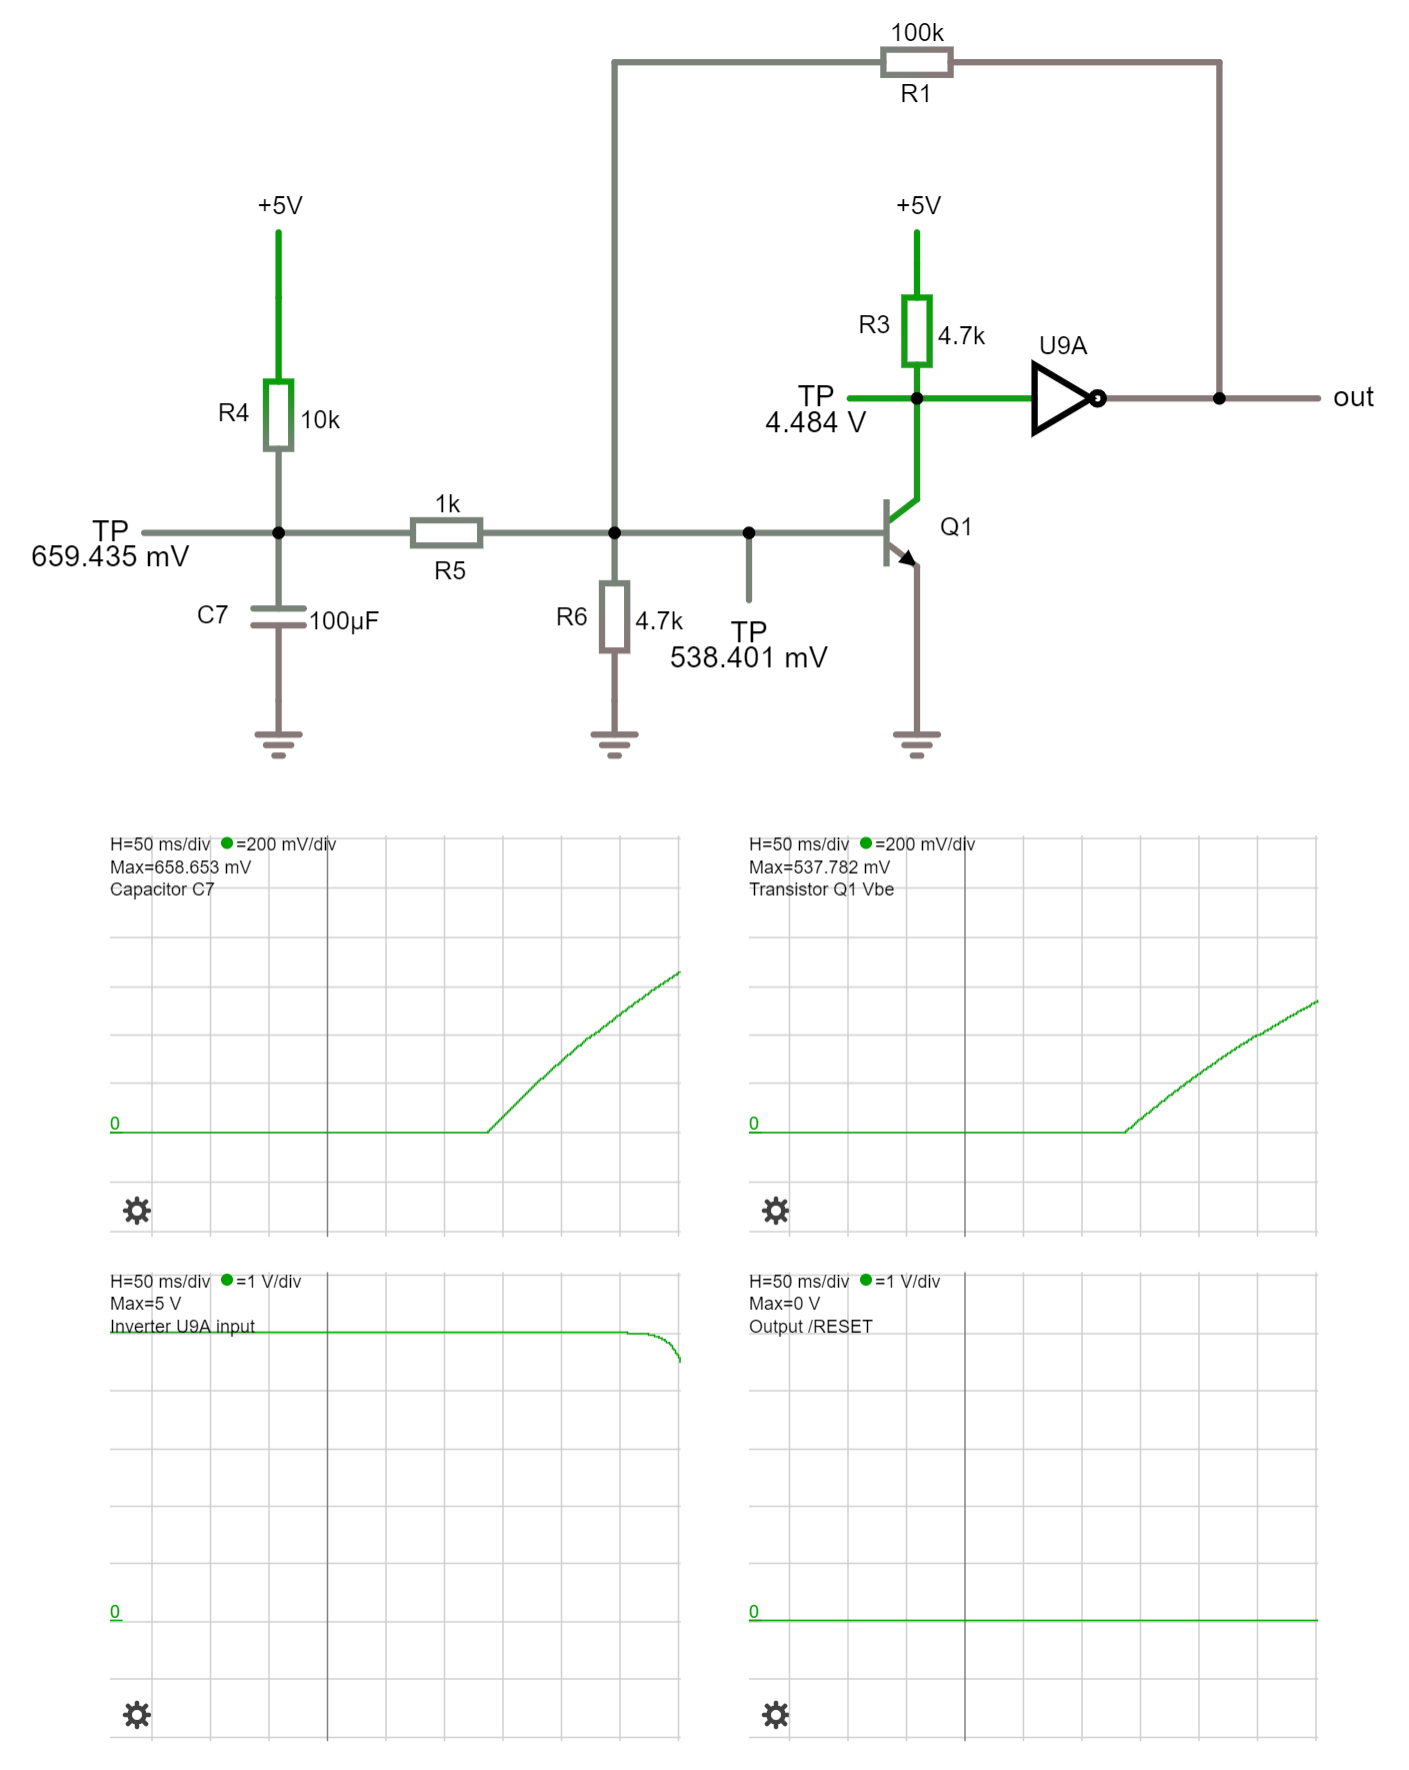
\includegraphics[width=0.7\linewidth]{figures/simul-por-02}
  \caption{Simulation of Power-On Reset: the capacitor {\tt C7} initiates its charge cycle}
  \label{fig:simul-por-02}
\end{figure}

As the current is flowing, it will initiate the charging cycle of the capacitor, what requires some time to complete. During that time, it will be draining the current coming from the power supply throught {\tt R4}. And the voltage in its positive terminal will increase slowly, following a loading curve shown in the top-left graph of the simulation in Figure \ref{fig:simul-por-02}.

As the time passes, the capacitor will increase its charge and voltage. And that will also increase the current going through {\tt R5} and {\tt R6}. Part of this current will go through the base terminal of the transistor {\tt Q1}, making it leave the cut-off region to enter the active region. This is shown in the top-right graph of the simulation in Figure \ref{fig:simul-por-02}.

When this happens, the collector-emitter current will be the base current amplified by the transistor gain: $I_C = h_{FE} \cdot I_B$. This will cause a voltage drop in {\tt R3} due to that current, with an interesting side effect: the voltage at the input terminal of {\tt U9A} will be reduced. This is shown in the bottom-left graph of the simulation in Figure \ref{fig:simul-por-02}.

At this moment, the collector current is still too low to cause a significant voltage drop in {\tt R3}. Thus, the voltage at the input of {\tt U9A} is still above the transition level. As consequence, the output of {\tt U9A} is still low. This is shown in the bottom-right graph of the simulation in Figure \ref{fig:simul-por-02}.

So in summary, the voltage of the input terminal of {\tt U9A} is inversely proportional to the charge of the capacitor {\tt C7}. The more charge in the capacitor, the less voltage in the logic inverter.

Approximately 100ms after power on, the situation changes to that represented in the simulation shown in Figure \ref{fig:simul-por-03}.

\begin{figure}[htb]
  \centering
  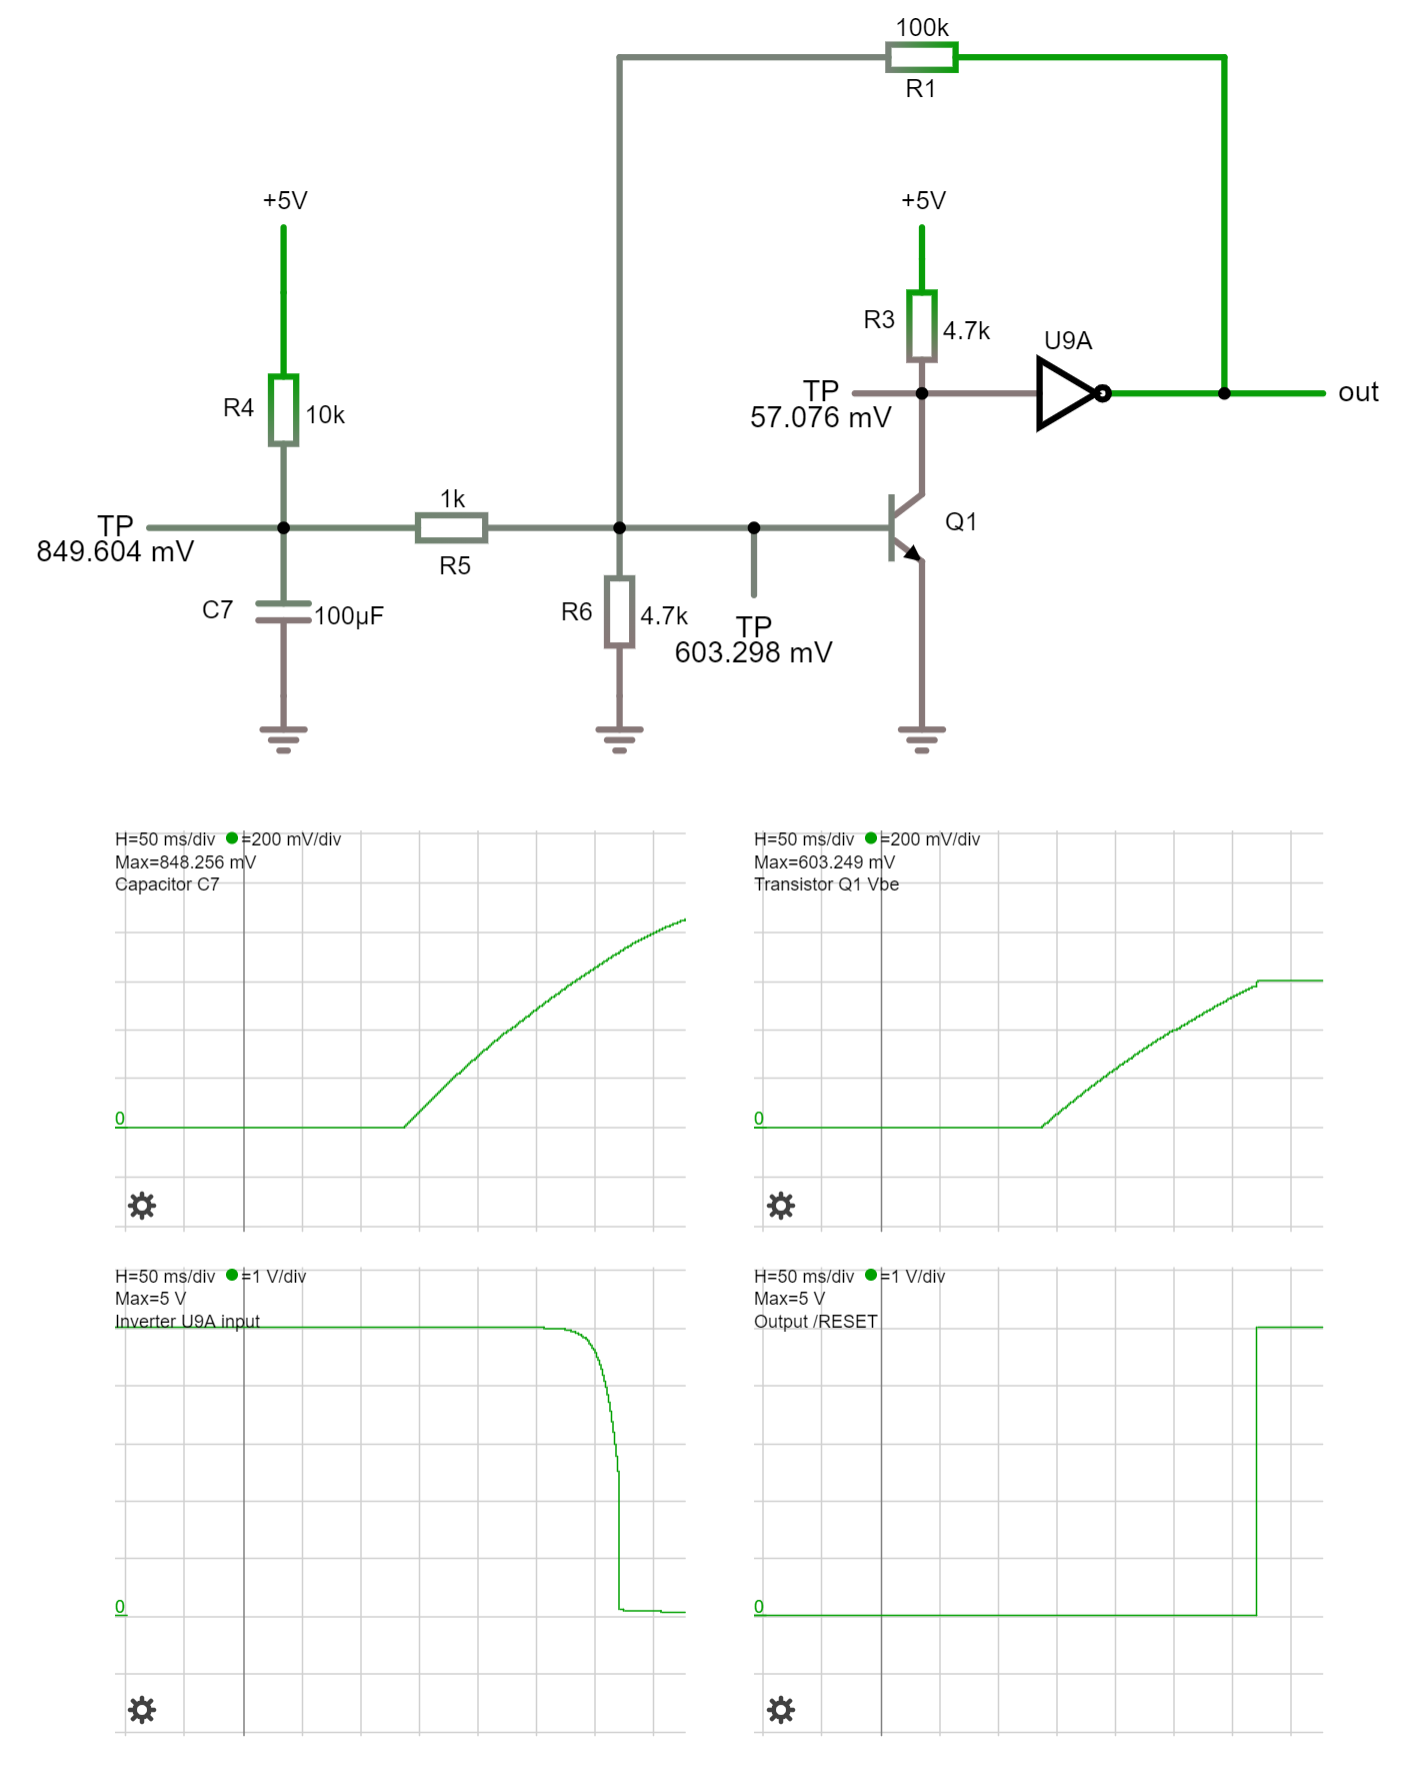
\includegraphics[width=0.7\linewidth]{figures/simul-por-03}
  \caption{Simulation of Power-On Reset: the charge of {\tt C7} causes a transition in {\tt U9A}}
  \label{fig:simul-por-03}
\end{figure}

The charge in {\tt C7} has been increased following its charge curve. This is shown in the top-left graph of the simulation of Figure \ref{fig:simul-por-03}.

As consequence, the transistor {\tt Q1} pushes more and more current through its collector. This is shown in the top-right graph of the simulation of Figure \ref{fig:simul-por-03}.

The collector current in the transistor causes a voltage drop in {\tt R3} that reduces the voltage at the input of {\tt U9A} below the transition level. This is shown in the bottom-left graph of the simulation of Figure \ref{fig:simul-por-03}.

Once the input of {\tt U9A} falls below some mid-point level, the inverter will transit into a new state. The output will change from logic low to high. This is shown in the bottom-right graph of the simulation of Figure \ref{fig:simul-por-03}.

The rest of inverters {\tt U9B} and {\tt U9C} will change their state as well. So the level of {\tt RESET} will pass to be low and the level of {\tt /RESET} will pass to be high. That is the effective termination of the reset pulse.

However, that is not all. If you look carefully the graphs in Figure \ref{fig:simul-por-03}, you may find something odd. The voltage at the input of {\tt U9A} falls abruptly to zero just after it reaches the mid-point where level transition occurs. In turn, there is also a drastic increment in the $V_{BE}$ of the transistor just before it reaches its top.

This effect is caused by the resistor {\tt R1}. This is a positive feedback loop that connects the output of {\tt U9A} to the base terminal of {\tt Q1}. And there is a good reason to make this. In fact, the Power-On Reset will not work without it!

When input voltage of an inverter is close to the mid-point, any small change in that input will be reflected with a huge change in the output. This is the point where voltage gain is maximum. Unfortunately, any electric wire has some amount of electrical noise that may cause small changes in its voltage, both positive and negative. When this happens in the input of the inverter when the voltage is close to the mid-point, the output could experiment huge oscillations.

This situation is represented in the simulation shown in Figure \ref{fig:simul-por-04}. This time we have altered the simulation to use a noisy power supply instead of perfectly unaltered 5 volts as before. We have also removed the positive feedback loop.

\begin{figure}[htb]
  \centering
  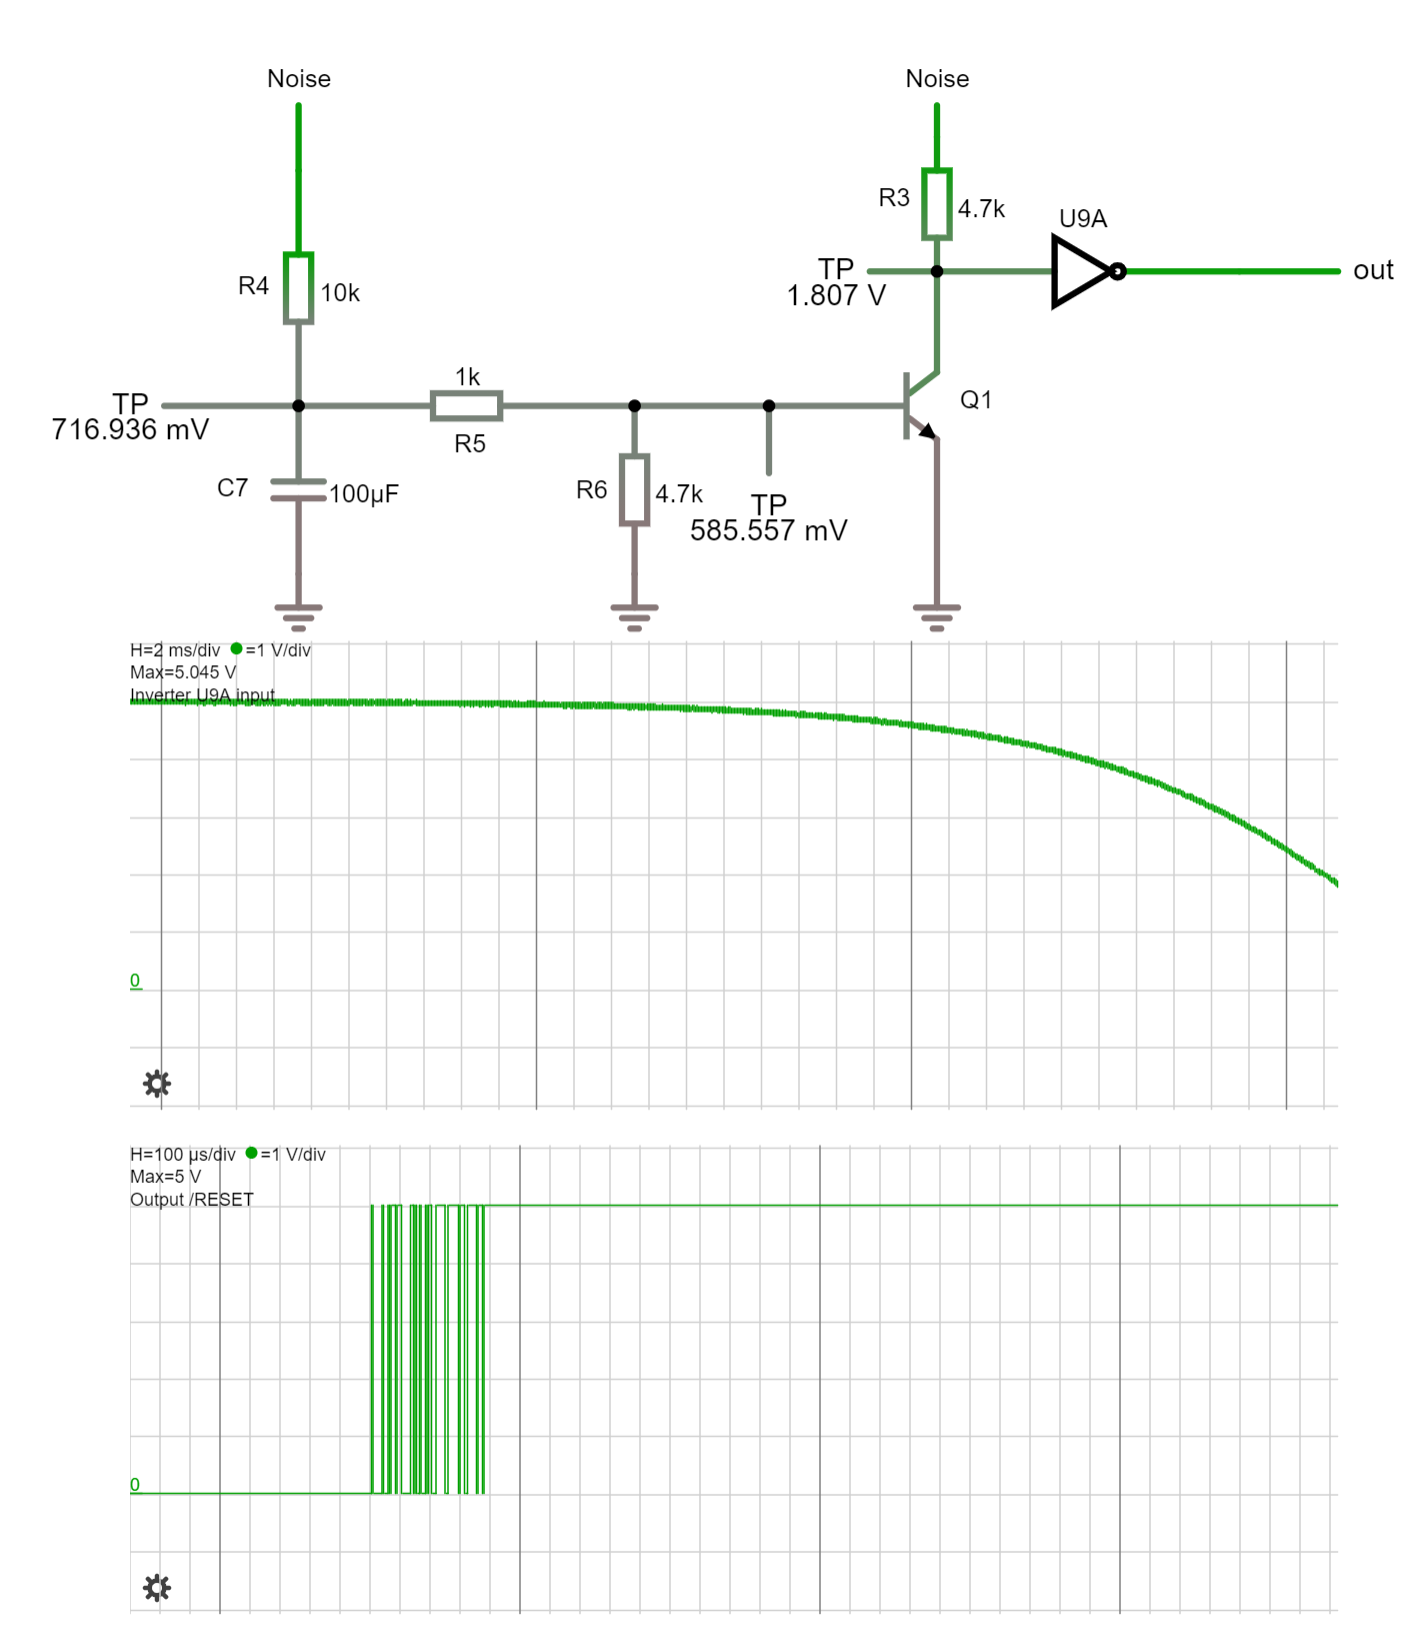
\includegraphics[width=0.7\linewidth]{figures/simul-por-04}
  \caption{Simulation of Power-On Reset: effect of removing the positive feedback loop}
  \label{fig:simul-por-04}
\end{figure}

As we can see in Figure \ref{fig:simul-por-04}, when the input voltage at {\tt U9A} reaches the mid-point (top graph), the noise in the line causes a few oscillations in the output (bottom graph). These oscillations would be interpreted by devices receiving the reset signal as a new reset action. However, they are too short in time. Just a few microseconds in the best case. Some devices as the Z80 CPU requires reset pulses of several milliseconds at minimum. This short and false pulses will left these devices into an inconsistent state. And your computer will not boot correctly.

In a standard logic circuit, this is not an issue due to how fast the signals transit between logic levels. Logic gates are made of transistors that do not respond immediately to the changes in their inputs, taking several nanoseconds to raise or fall one single volt in the output. Thus, if the input signal transition is in the range of nanoseconds, a small noise in the line will not be reflected.

However, in out circuit the input of {\tt U9A} changes very slowly. We can see in the simulation of Figure \ref{fig:simul-por-04} that it takes 40ms just to go from the top of voltage to the mid-point. This is what is known as a slow signal, and it will cause oscillations if they are not handled as we do with the positive feedback loop.

But, how the positive feedback loop is helping to remove the output oscillations? Easy. You can see how it happens in the simulation shown in figure \ref{fig:simul-por-05}.

\begin{figure}[htb]
  \centering
  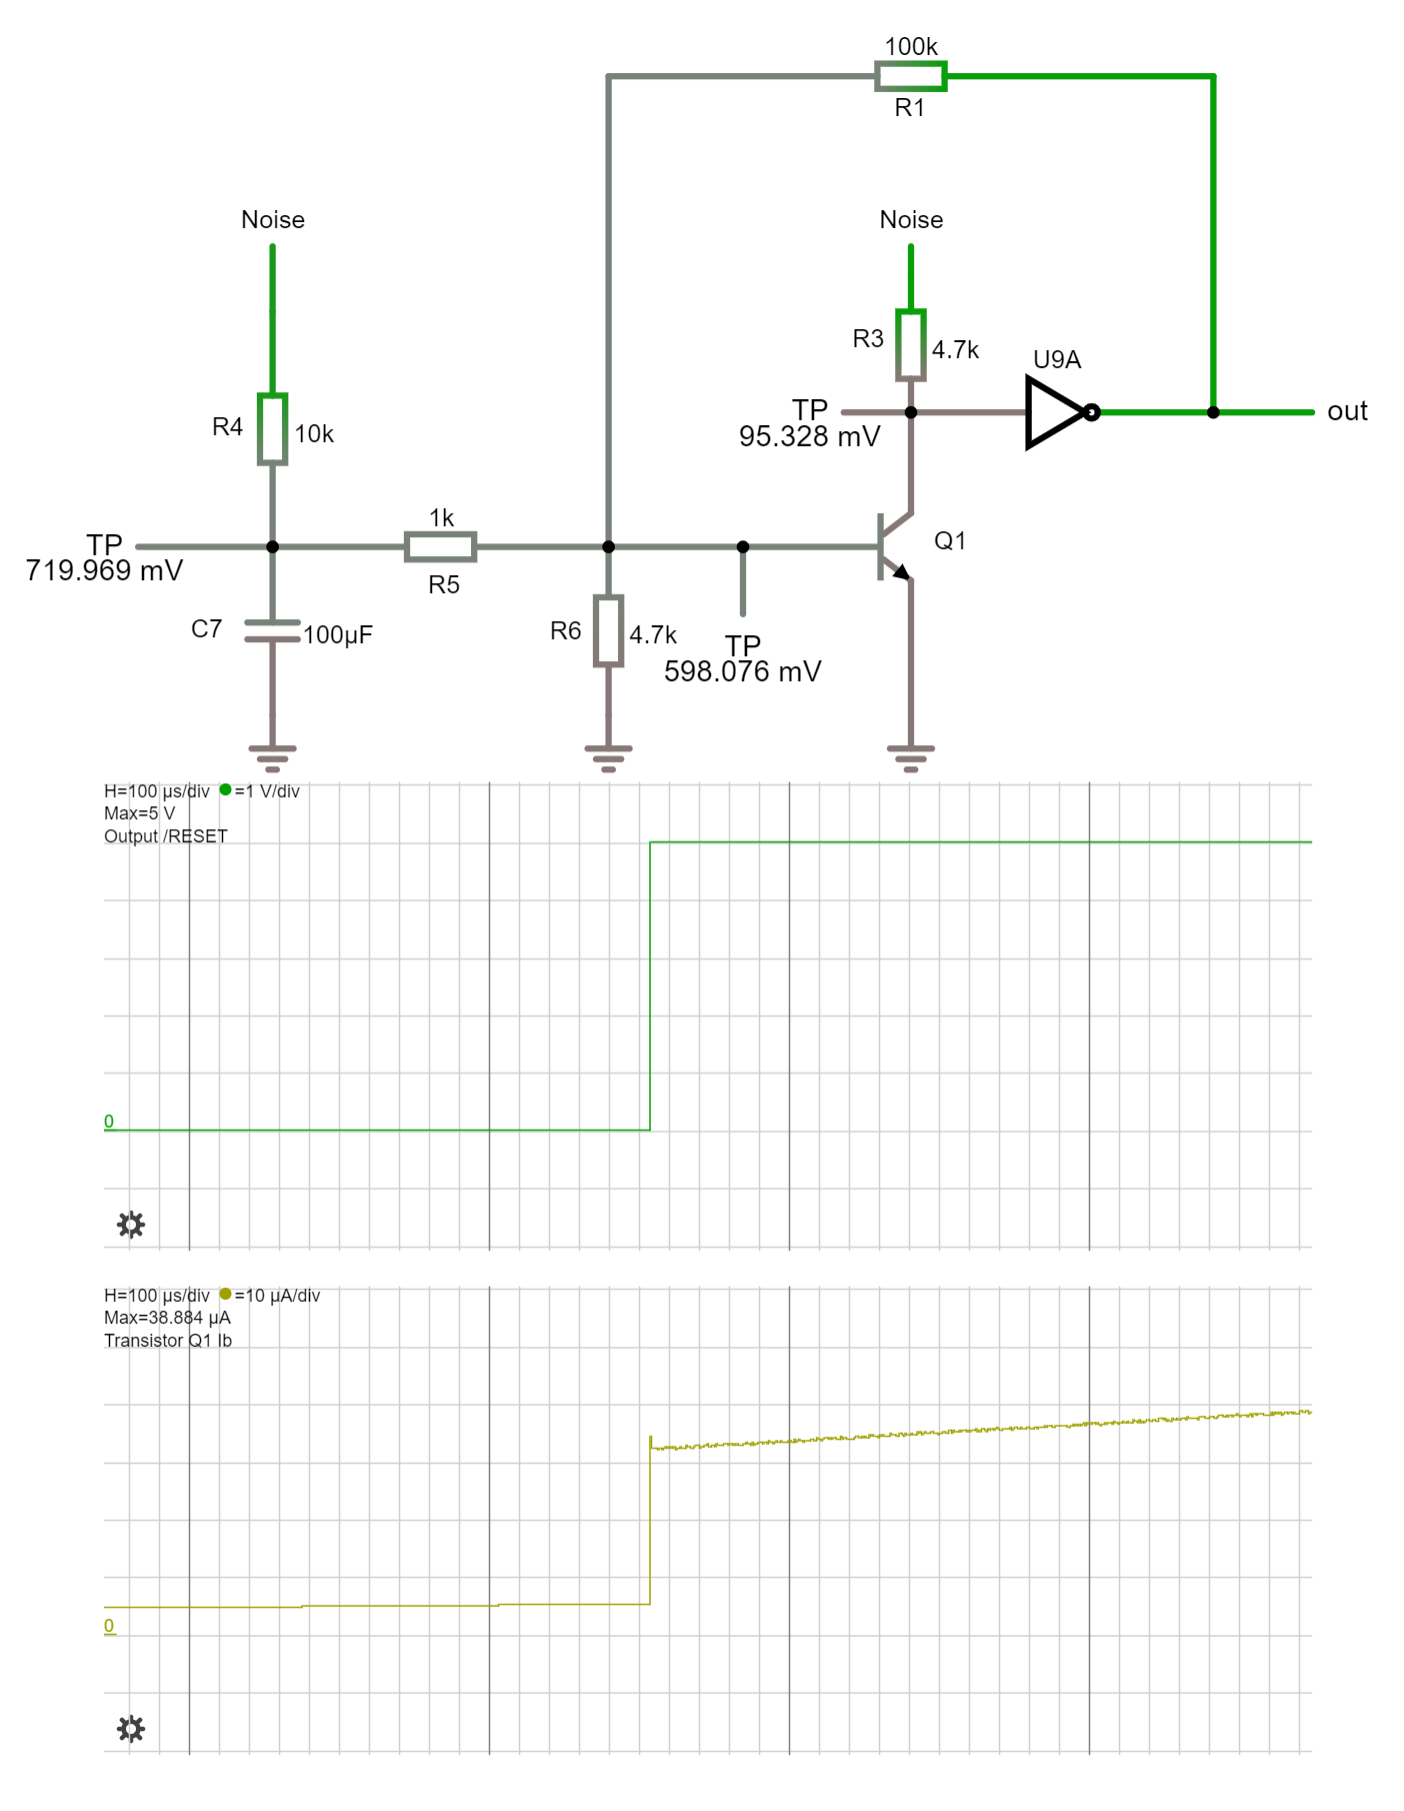
\includegraphics[width=0.7\linewidth]{figures/simul-por-05}
  \caption{Simulation of Power-On Reset: impact of positive feedback loop in $I_B$ of {\tt Q1}.}
  \label{fig:simul-por-05}
\end{figure}

The first transition from low to high in the output of {\tt U9A} will drive a small current through {\tt R1}. Part of this current will join to the current coming from {\tt R5} to increase the $I_B$ of the transistor. And this increment is not small, as shown in bottom graph of Figure \ref{fig:simul-por-05}. It goes from 5 to 32 microamperes. This current is enough to put the transistor in the saturation region. What means an effective closed circuit between the collector and the emitter. This is what pulls the input voltage of {\tt U9A} to almost zero before the noise has time to cause any oscillation in the inverter.

There is some other thing in this circuit that also helps to mitigate the oscillations in the inverter. This is the usage of a {\tt 74HCU04} inverter instead of {\tt 74HC04}. That extra {\it U} in the part name means {\it unbuffered}.

One of the multiple particularities of unbuffered gates is that they have lower gains than their buffered equivalents. Unbuffered gates have a single amplifier phase, while buffered ones typically have three. Each phase increases the gain of the overall circuit. Thus, you might expect that unbuffered inverters have a maximum gain of a few hundreds, while buffered devices have several thousands.

Higher gain means they will react more drastically to the changes in their inputs. A tiny change in the input voltage caused by line noise will be reflected by an increment several orders of magnitude larger if the inverter is buffered. In other words, buffered gates are more sensible to line noise, specially when slow signals are used. Thus, this design uses {\tt 74HCU04} unbuffered inverters.

Now you know almost everything about a reliable Power-On Reset circuit. Everything but how an actual reset without a power-on can be done. This is achieved by switch {\tt SW1} and a diode {\tt D1} shown at the left side of the circuit of Figure \ref{fig:artemisa-schematic-por}.

The diode is used to discharge the capacitor {\tt C7} quickly when the power is disconnected. When that happens, the {\tt 5+} power will not drive 5 volts any longer, and it can drain the charge of the capacitor going through {\tt D1}. If this diode is not present, it would be possible to disconnect the power adapter and connect it again fastly. Fast enough to maintain the charge of the capacitor, and not having any reset signal. Thanks to the diode, the capacitor {\tt C7} is discharged very quickly as soon as the power adapter is unplugged from the DC barrel connector.

However, having to reconnect the power adapter everytime we want to reset the system is annoying. To avoid this pain in the ass, we have the switch {\tt SW1}. This switch connects the positive terminal of capacitor {\tt C7} to ground. When unpressed, this circuit is open. Upon press, the capacitor will discharge very quickly. This will return to the same state we had when the system was powered on. And a new reset pulse will begin.

Now we can say that is all. You have far enough to understand how the power connector and power-on reset circuits work. It is time to heat up the solder iron.

\section{Circuit assembly}

\subsection{Power connector}

We will start assembling the parts of the power connector circuit shown in Figure \ref{fig:artemisa-schematic-power-conn}.

\begin{enumerate}
  \item Solder the barrel power connector {\tt J1}. Its exact placement is shown in Figure \ref{fig:mount-power-01}.
  \item Solder the decoupling capacitors {\tt C5} and {\tt C6}. Their exact placement is shown in Figure \ref{fig:mount-power-02}.

        \begin{warning}[Be careful with the polarity of the electrolytic capacitors!]
          These capacitors are electrolytic, and they have a polarity. Please check you are soldering the right pads into the right holes. The long pad of the capacitor is the positive terminal. The short pad, which is also marked with a grey mark with minus symbols on the capacitor body, is the negative terminal.\\\\

          Soldering electrolytic capacitors with a reverse polarity may cause them to explode!
        \end{warning}
  \item Solder the resistor {\tt R2} and the LED {\tt D2}. Their exact placement is shown in Figure \ref{fig:mount-power-03}. Take care of the polarity of the LED. The long pad is the anode, and must be soldered in the hole with the plus sign mark. The short pad, which also have a notch in the base of the LED body, is the cathode, and must be soldered in the hole marked with the minus sign.
\end{enumerate}

\begin{figure}[htbp]
  \centering
  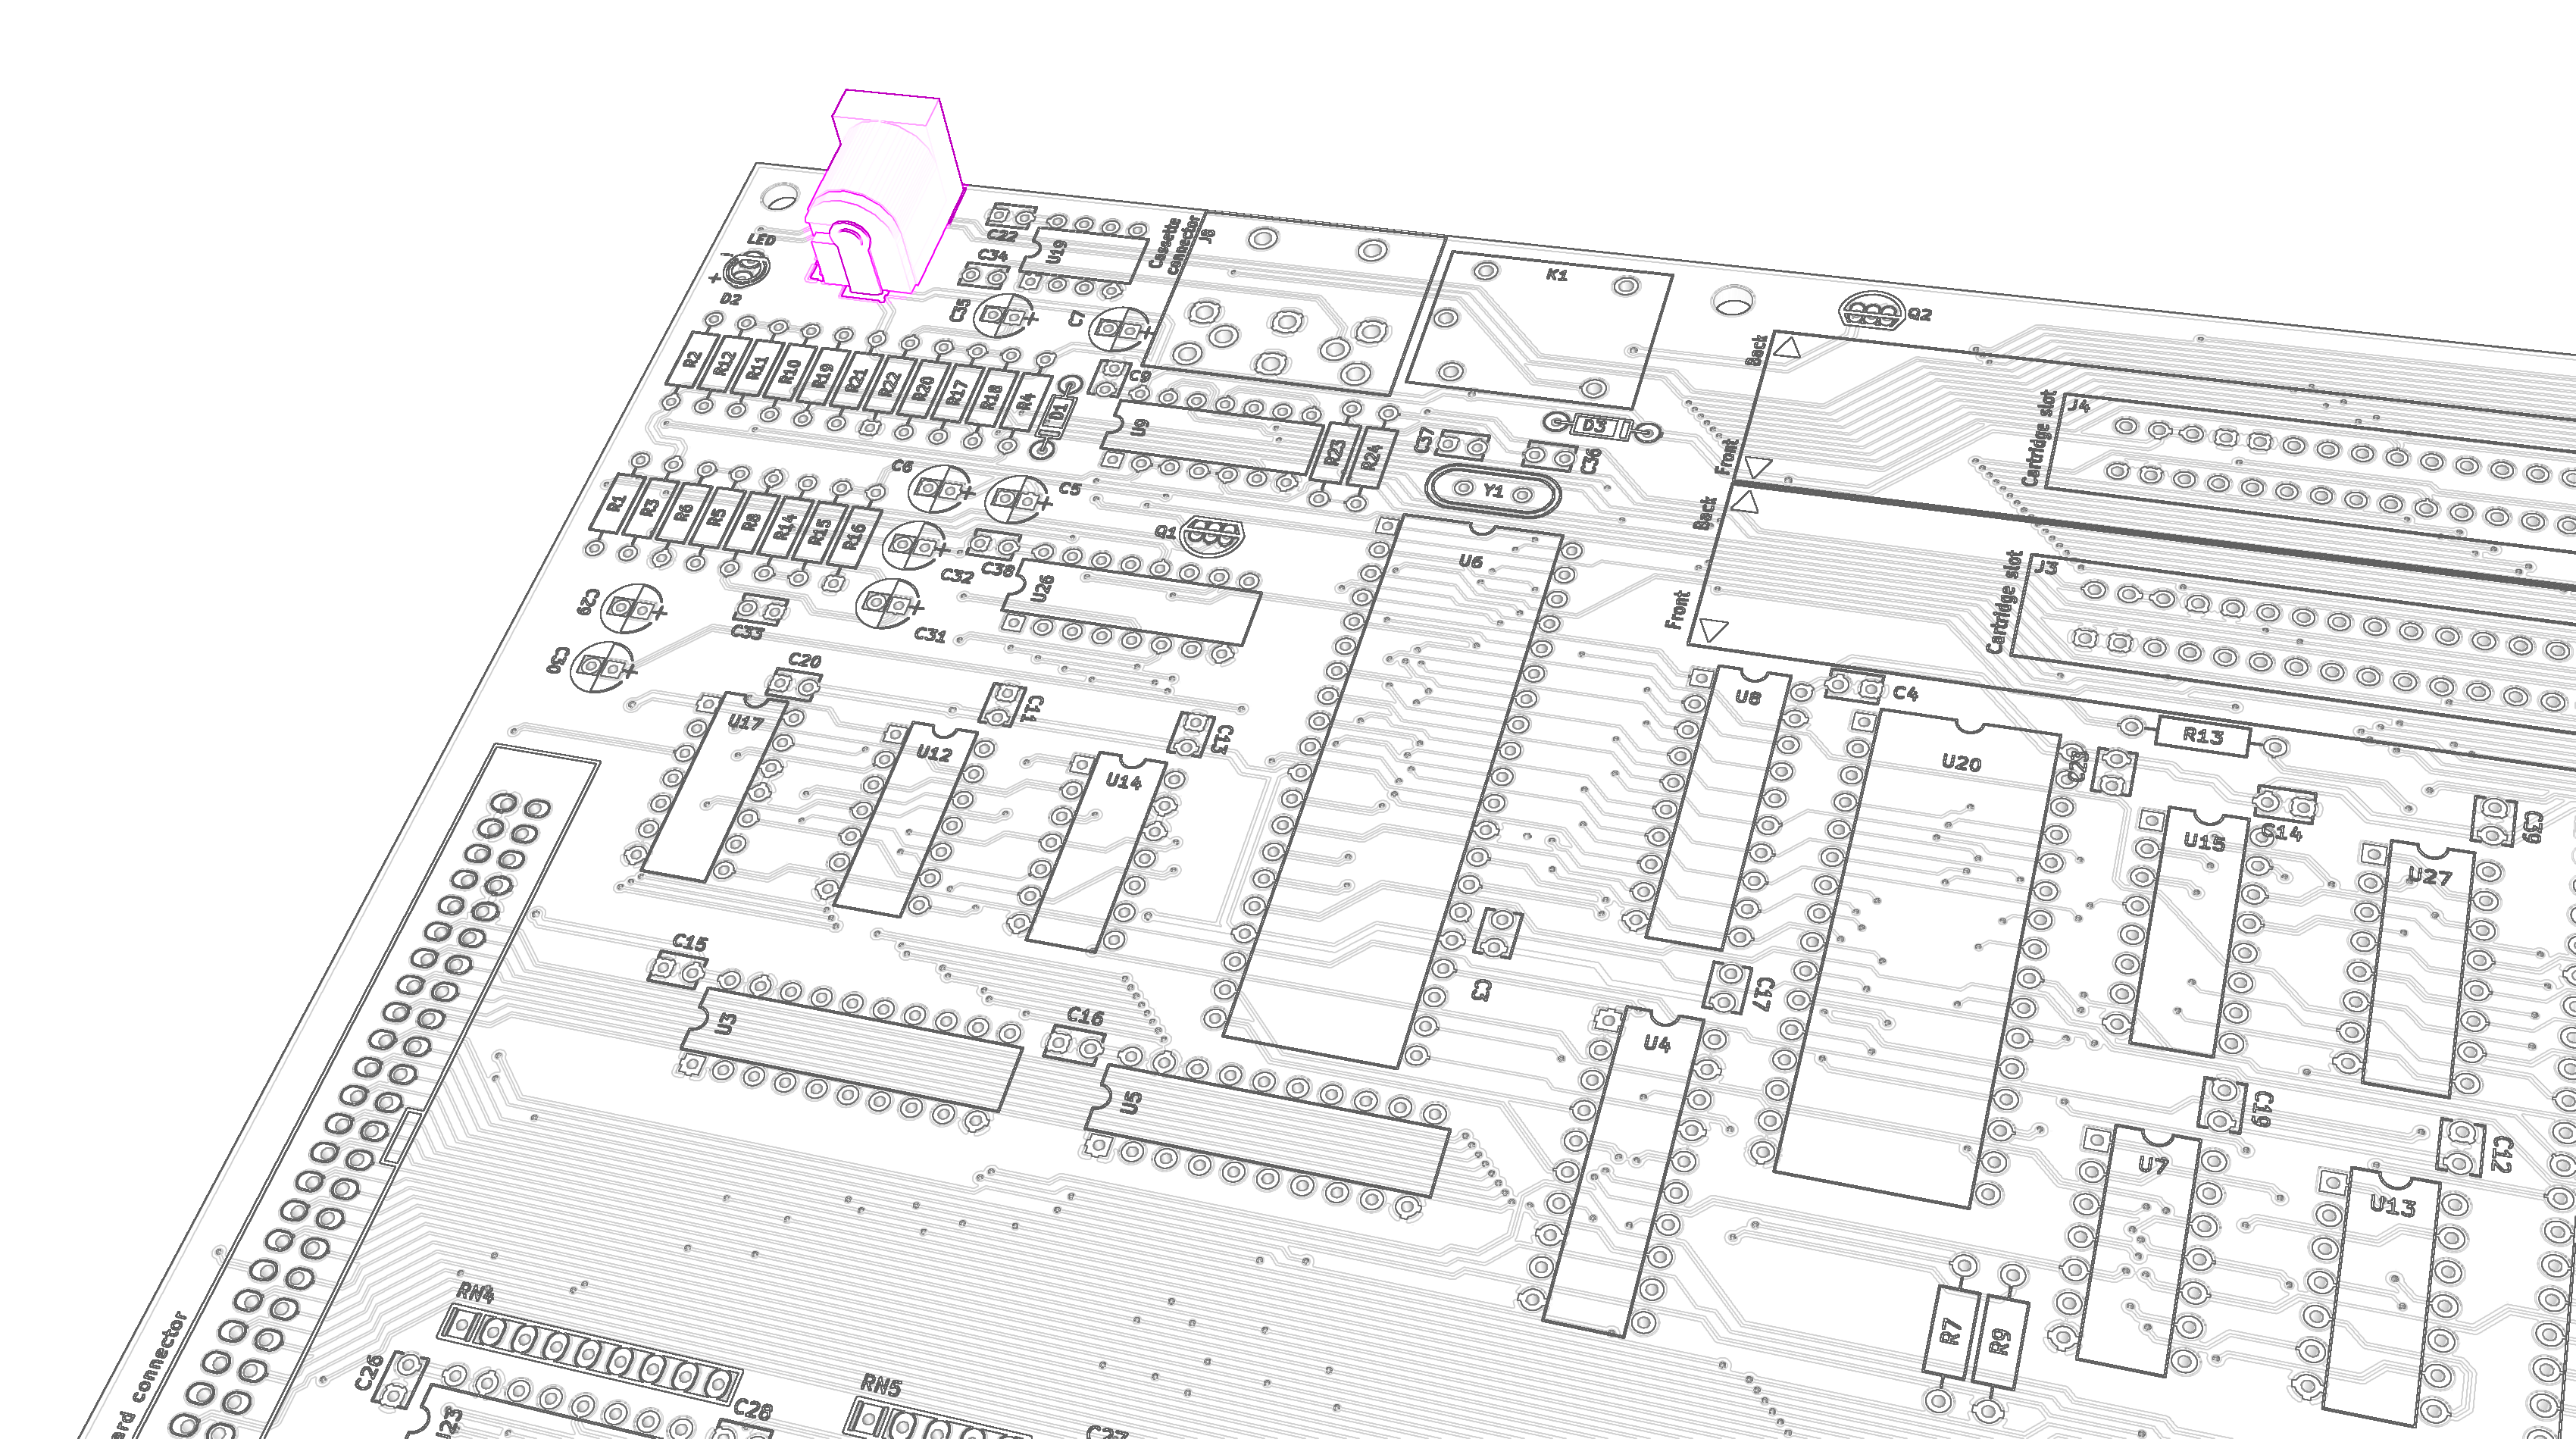
\includegraphics[width=0.8\linewidth]{figures/mount-power-01}
  \caption{Placement of power barrel connector {\tt J1}}
  \label{fig:mount-power-01}
\end{figure}

\begin{figure}[htbp]
  \centering
  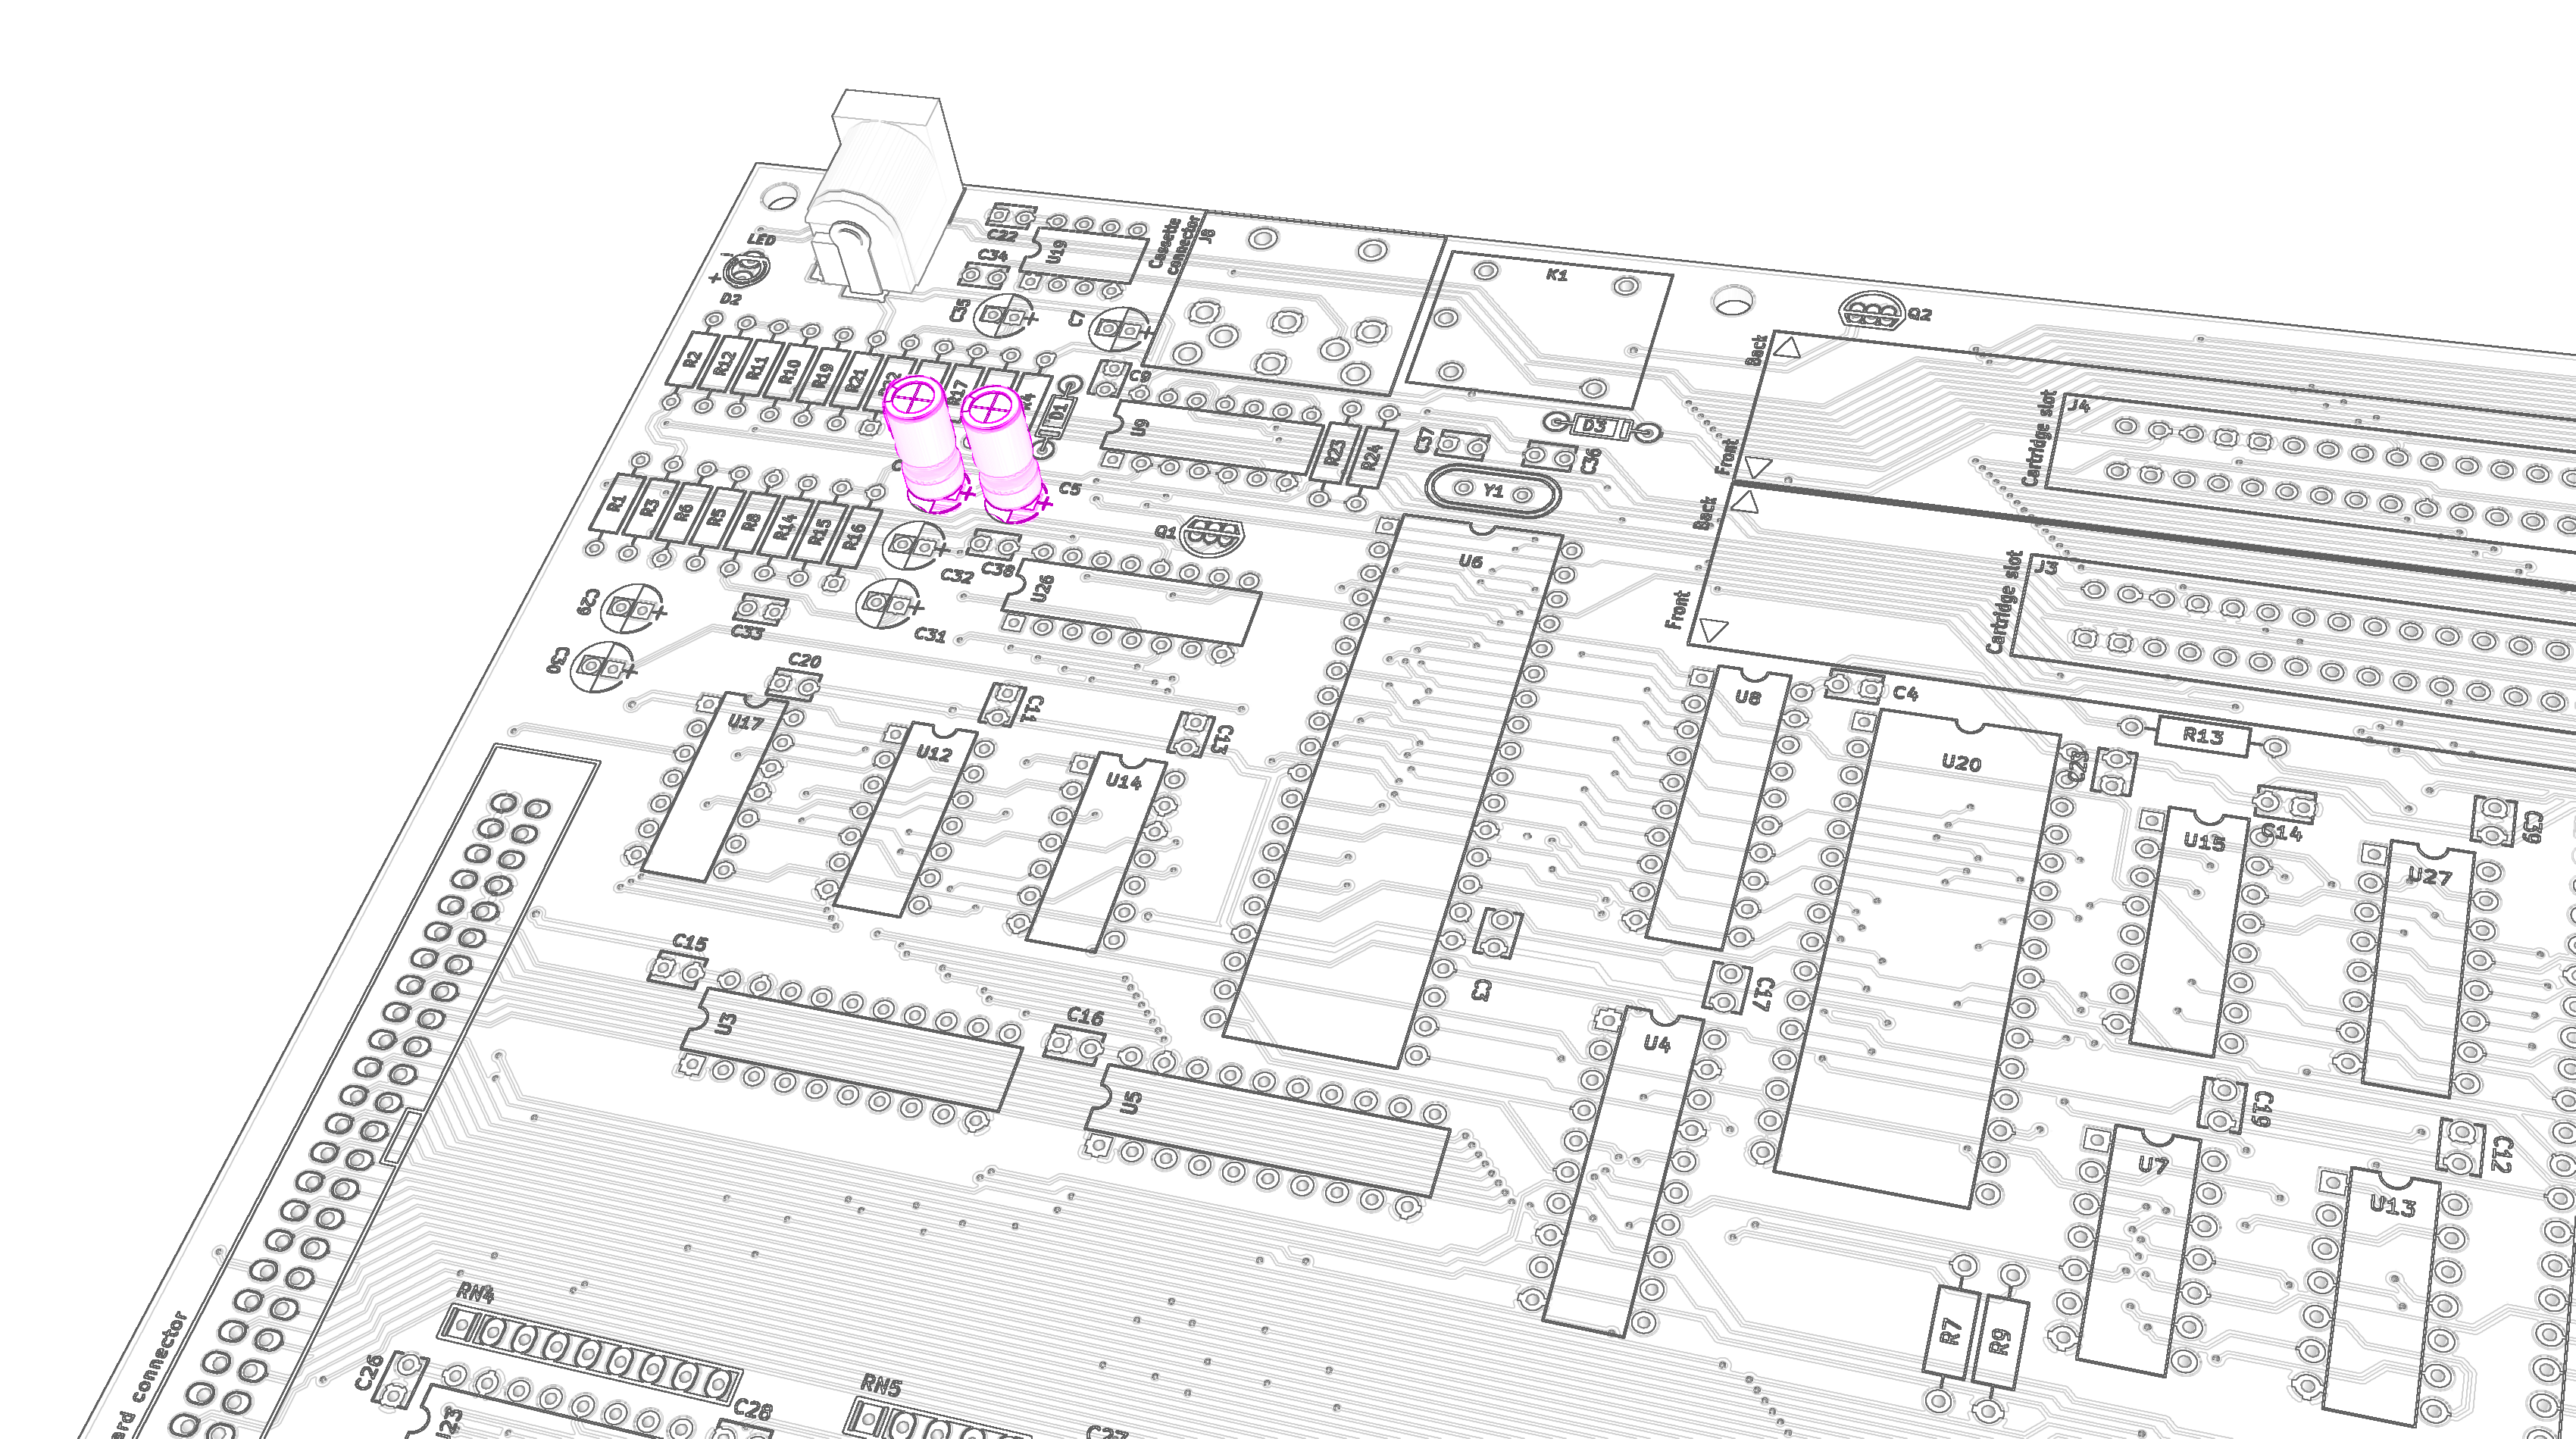
\includegraphics[width=0.8\linewidth]{figures/mount-power-02}
  \caption{Placement of decoupling capacitors {\tt C5} and {\tt C6}}
  \label{fig:mount-power-02}
\end{figure}

\begin{figure}[htbp]
  \centering
  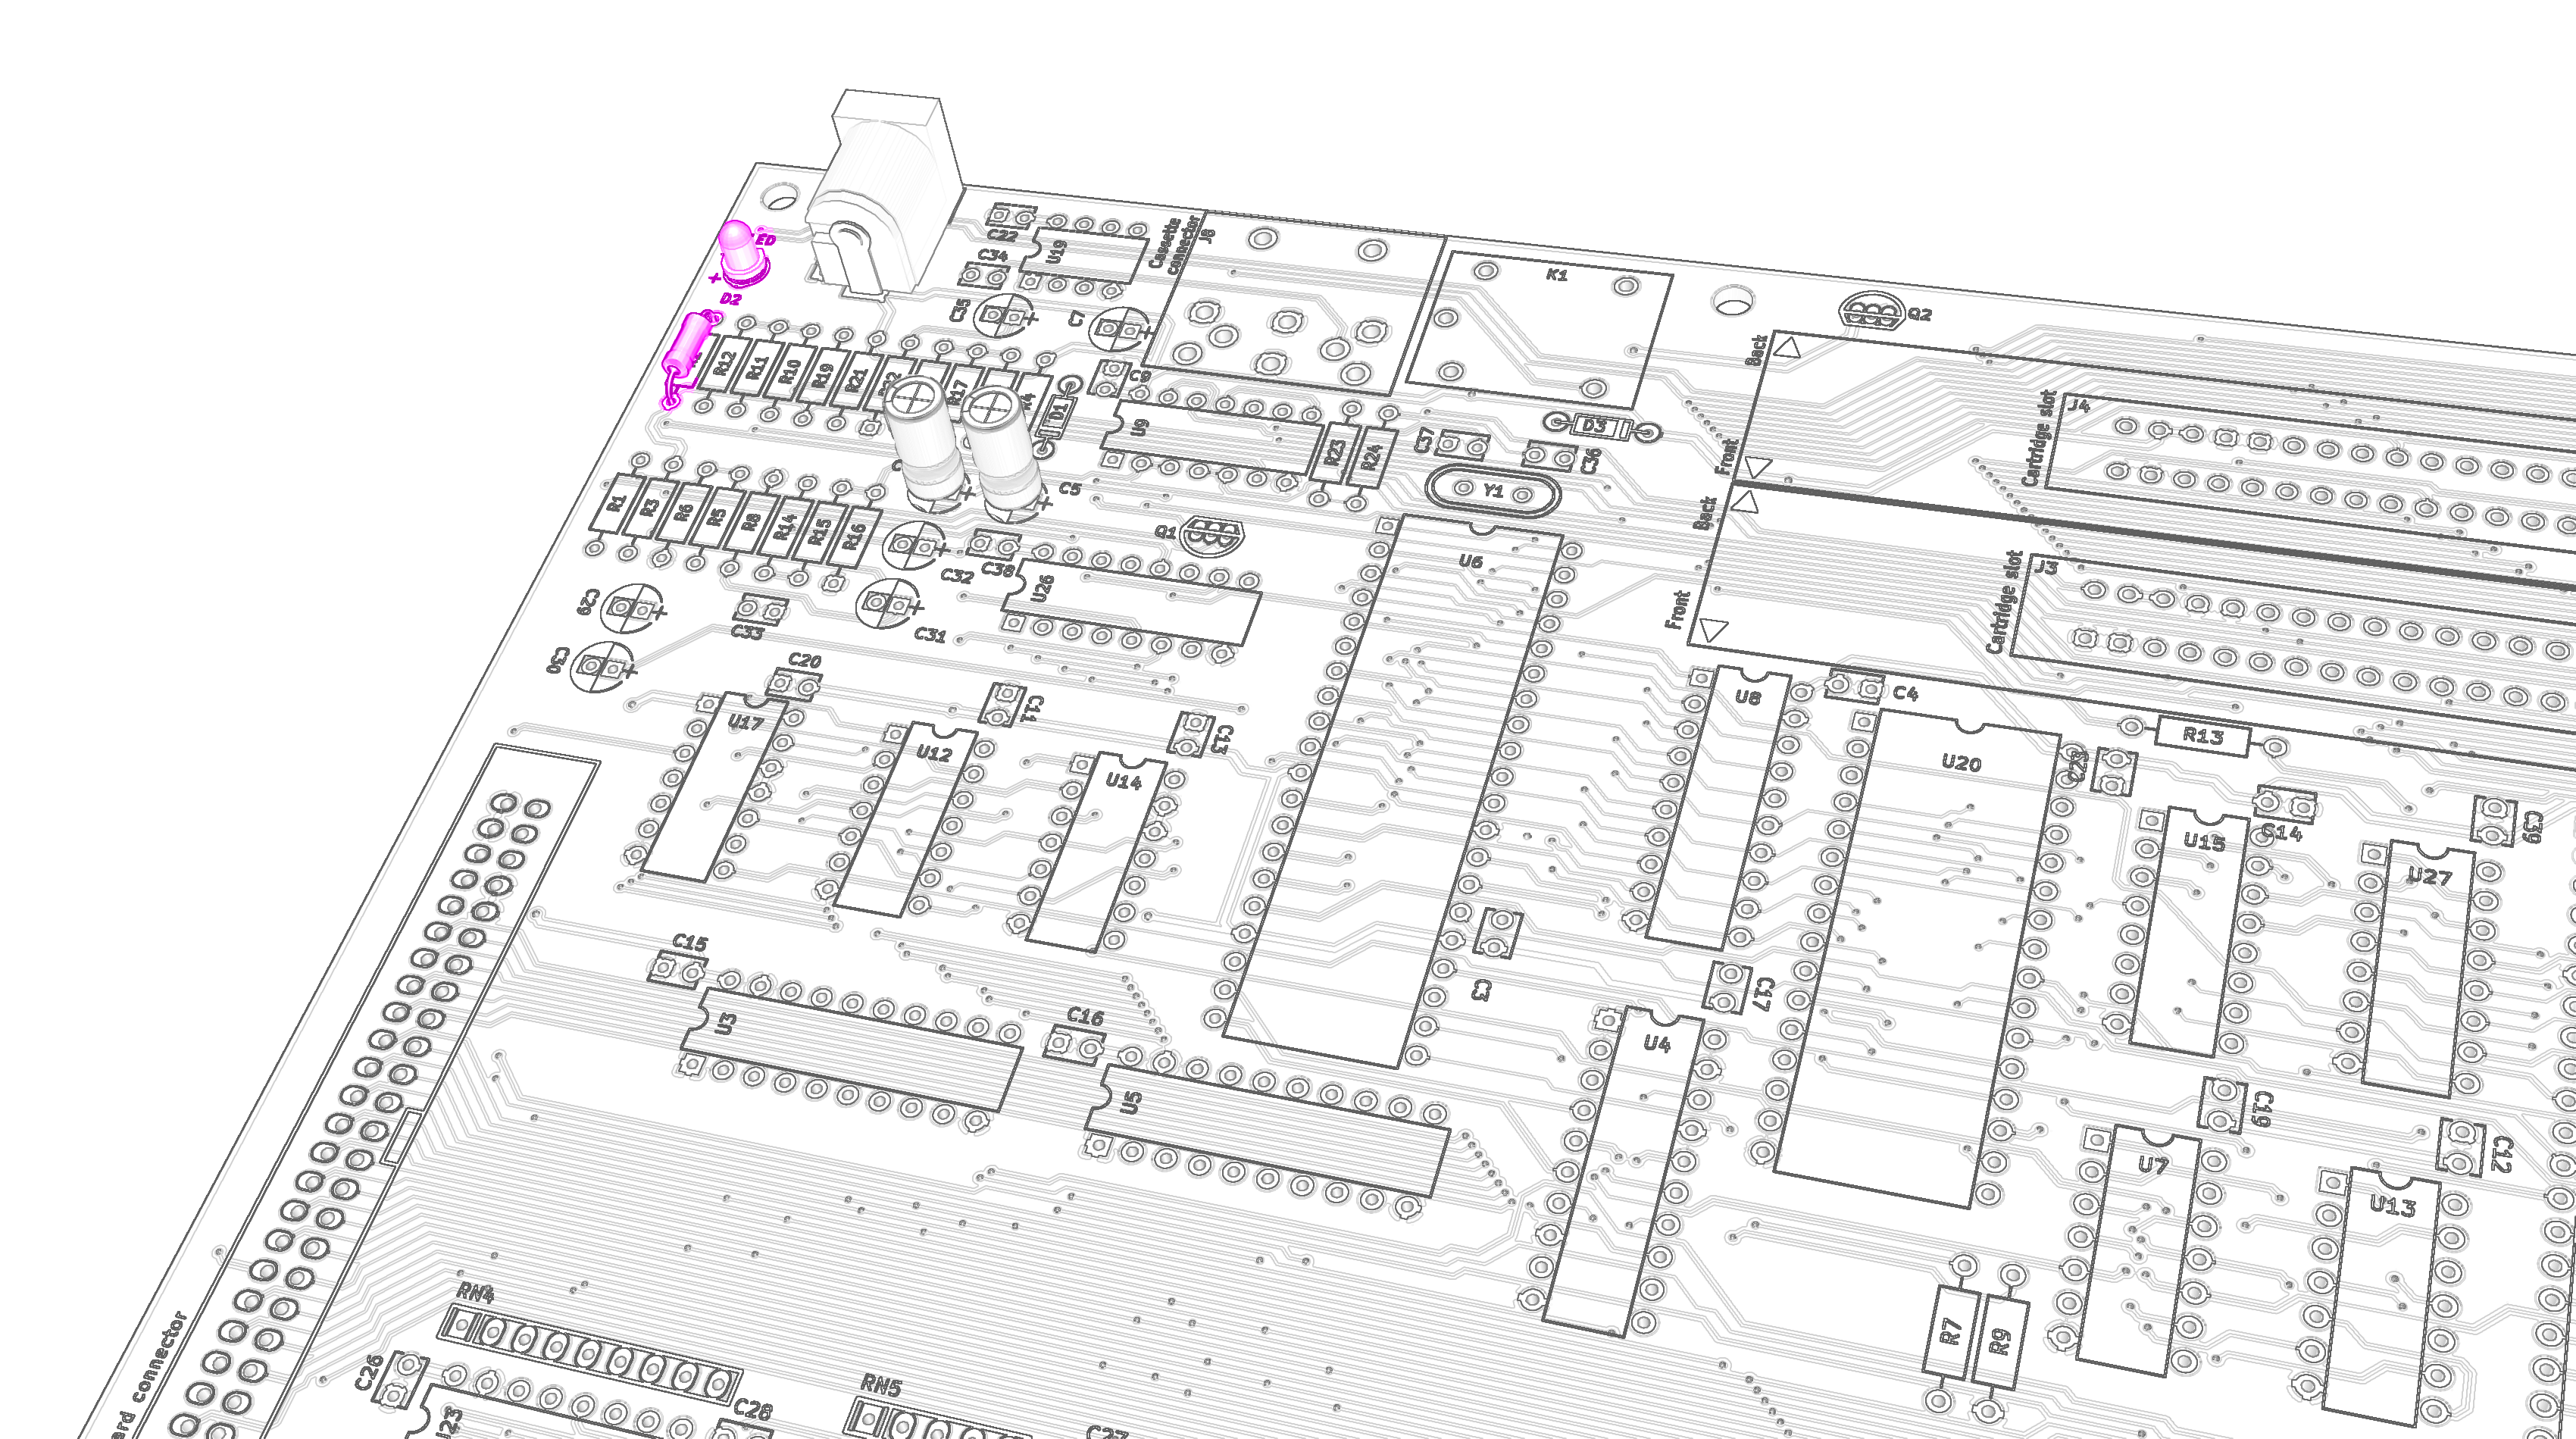
\includegraphics[width=0.8\linewidth]{figures/mount-power-03}
  \caption{Placement of resistor {\tt R2} and the LED {\tt D2}}
  \label{fig:mount-power-03}
\end{figure}

Once all the parts from the power circuit are assembled, it is time to test it:

\begin{enumerate}
  \item Connect the power adapter cable to the DC barrel connector. If everything goes well, the power LED will illuminate.
  \item If you have a multimeter, you can measure the DC voltage between the positive and negative terminals of the barrel connector. They should indicate a typical value of 5.00 volts. Any value from 4.75 to 5.25 volts is correct.
  \item Try to disconnect the power adapter cable. You will see the power LED is still illuminated. This is because the capacitors {\tt C5} and {\tt C6} are charged and they are feeding the LED. After a few seconds, the power drained by the LED circuit will discharge the capacitors and the LED will fade.
\end{enumerate}

\subsection{Power-On Reset}

Now we have the power sources assembled, it is time to go with the Power-On Reset circuit described in Figure \ref{fig:artemisa-schematic-por}.:

\begin{enumerate}
  \item Solder the resistors {\tt R4}, {\tt R5}, {\tt R6} and {\tt R1}. Their exact placement is shown in Figure \ref{fig:mount-power-04}.
  \item Solder the capacitor {\tt C7}. Its exact placement is shown in Figure \ref{fig:mount-power-05}.
  \item Solder the diode {\tt D1}. Its exact placement is shown in Figure \ref{fig:mount-power-06}.
  \item Solder the transistor {\tt Q1}. Its exact placement is shown in Figure \ref{fig:mount-power-07}.
  \item Solder the reset push button {\tt SW1}. Its exact placement is shown in Figure \ref{fig:mount-power-08}.
  \item Solder the IC {\tt U9} and its decoupling capacitor {\tt C9}. Their exact placement is shown in Figure \ref{fig:mount-power-09}.
\end{enumerate}

\begin{figure}[htbp]
  \centering
  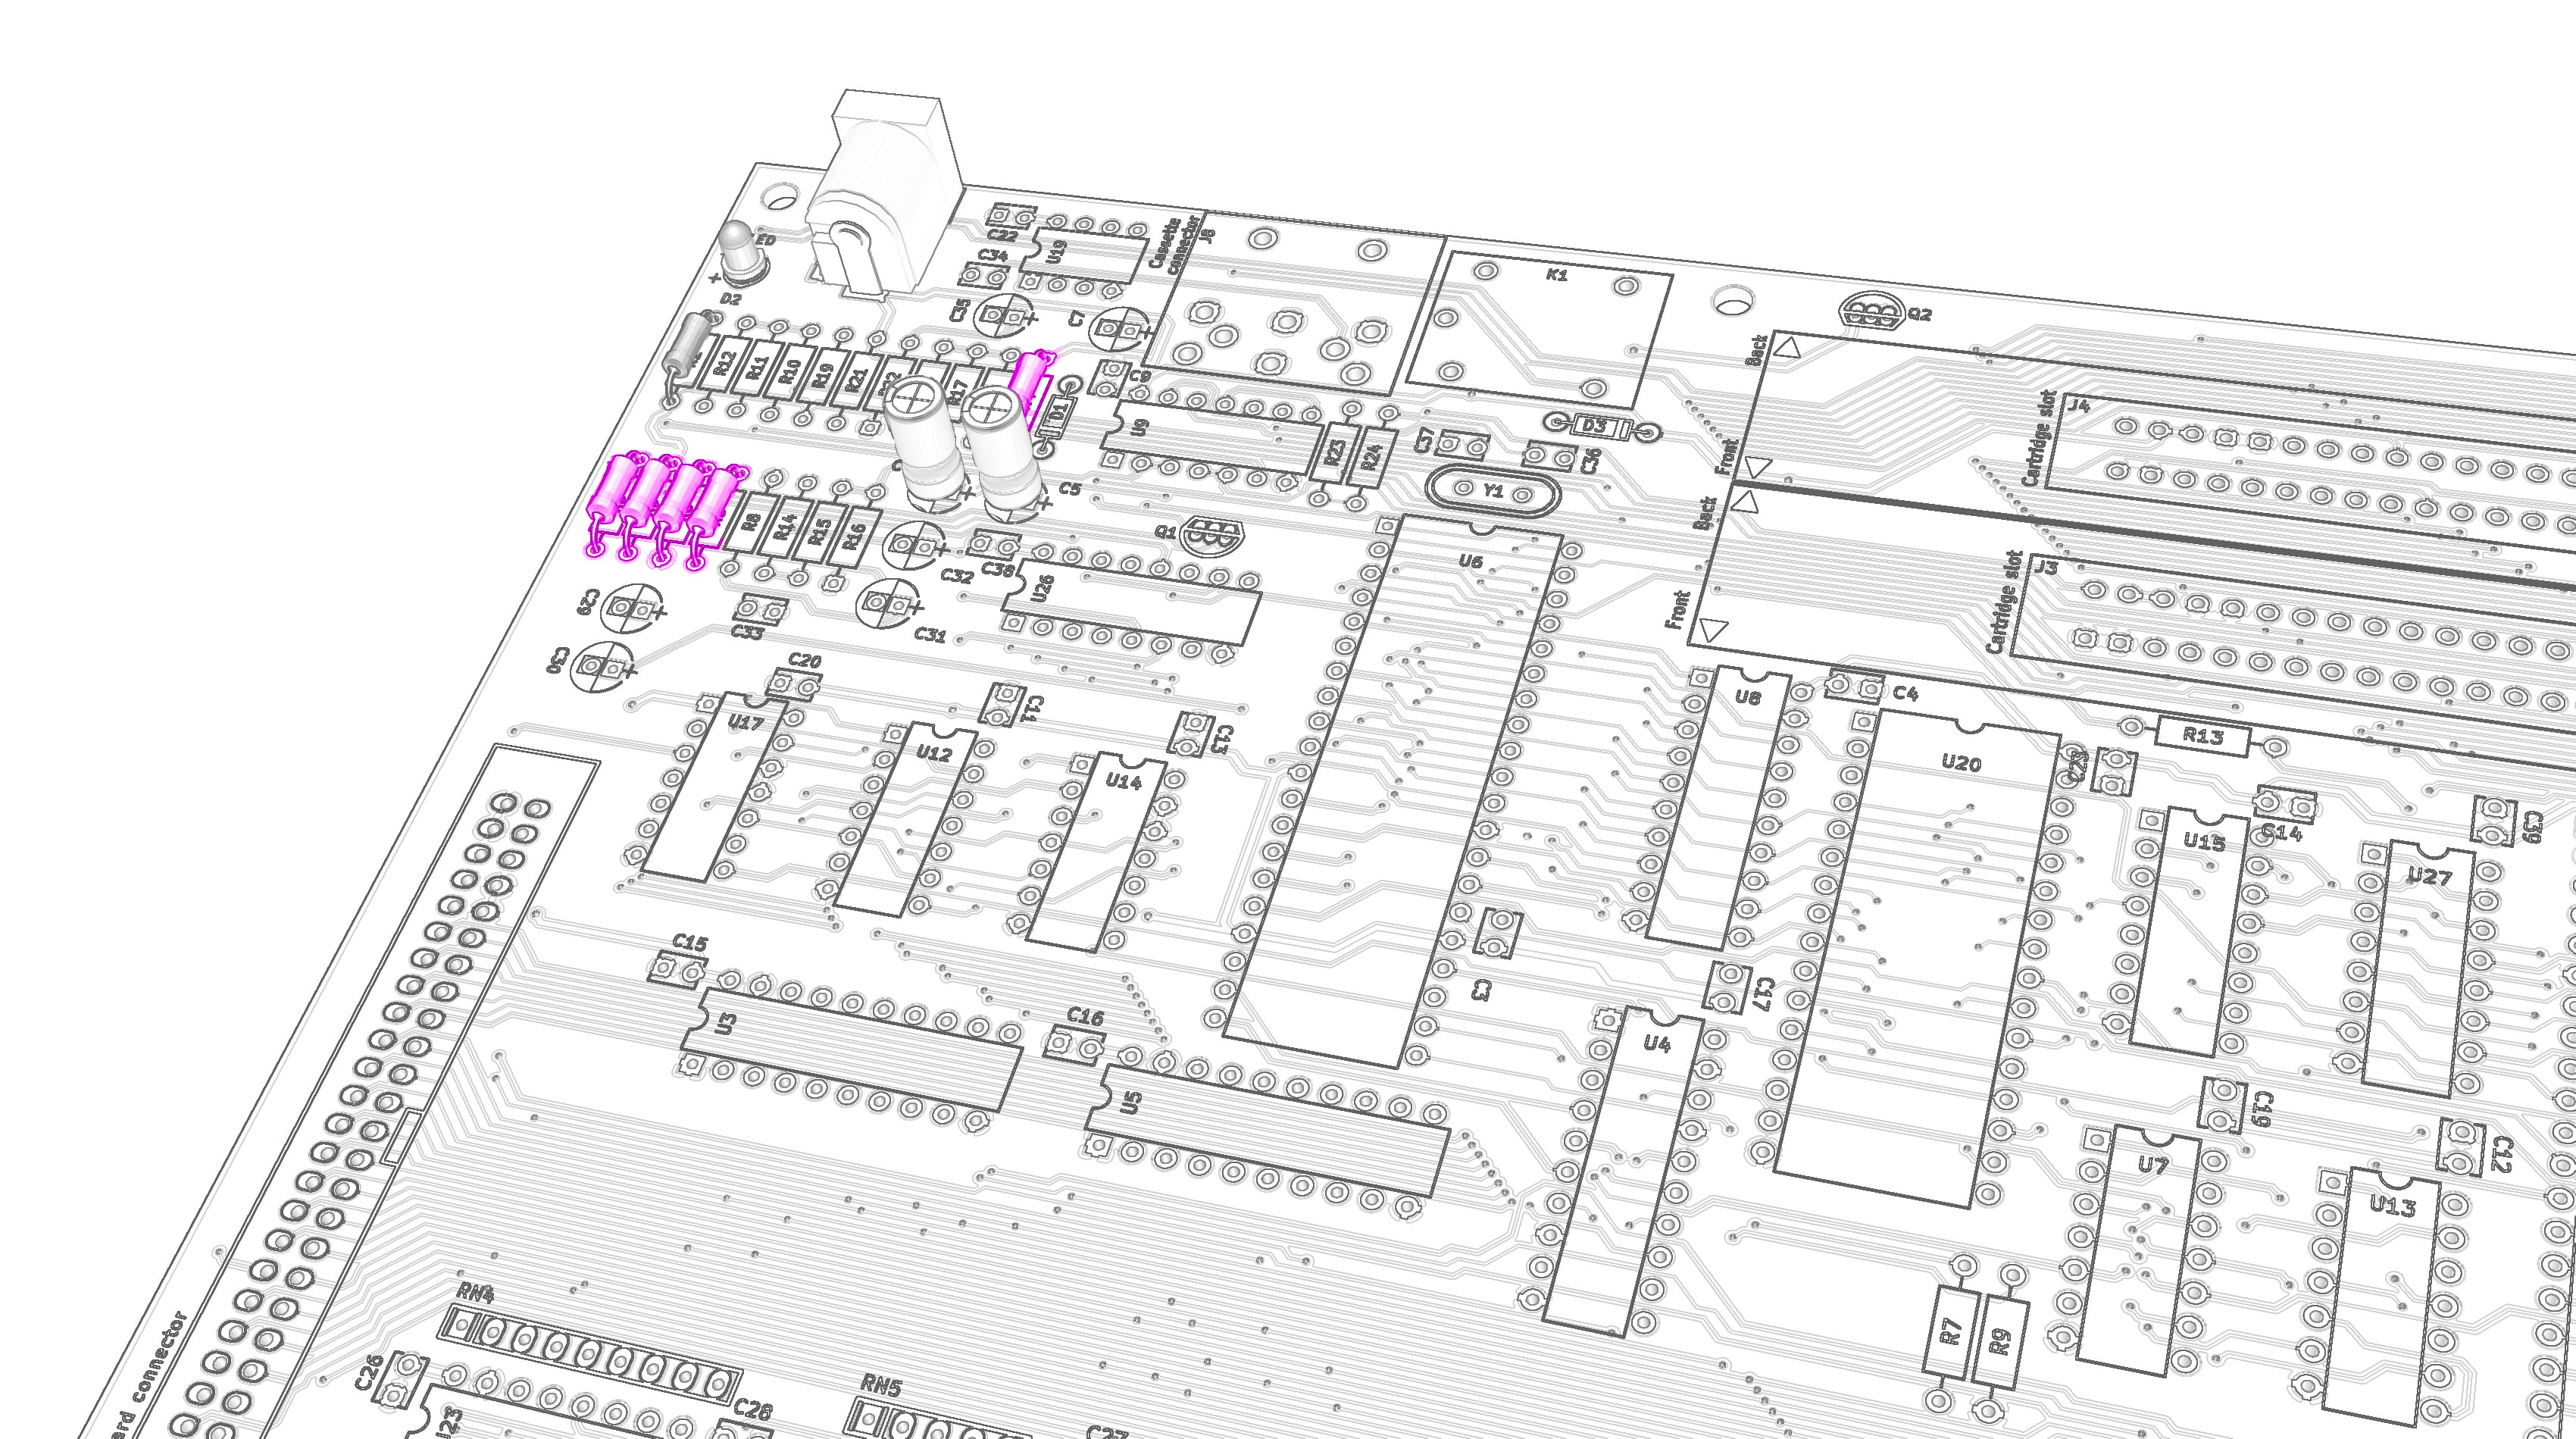
\includegraphics[width=0.8\linewidth]{figures/mount-power-04}
  \caption{Placement of resistors {\tt R4}, {\tt R5}, {\tt R6} and {\tt R1}}
  \label{fig:mount-power-04}
\end{figure}

\begin{figure}[htbp]
  \centering
  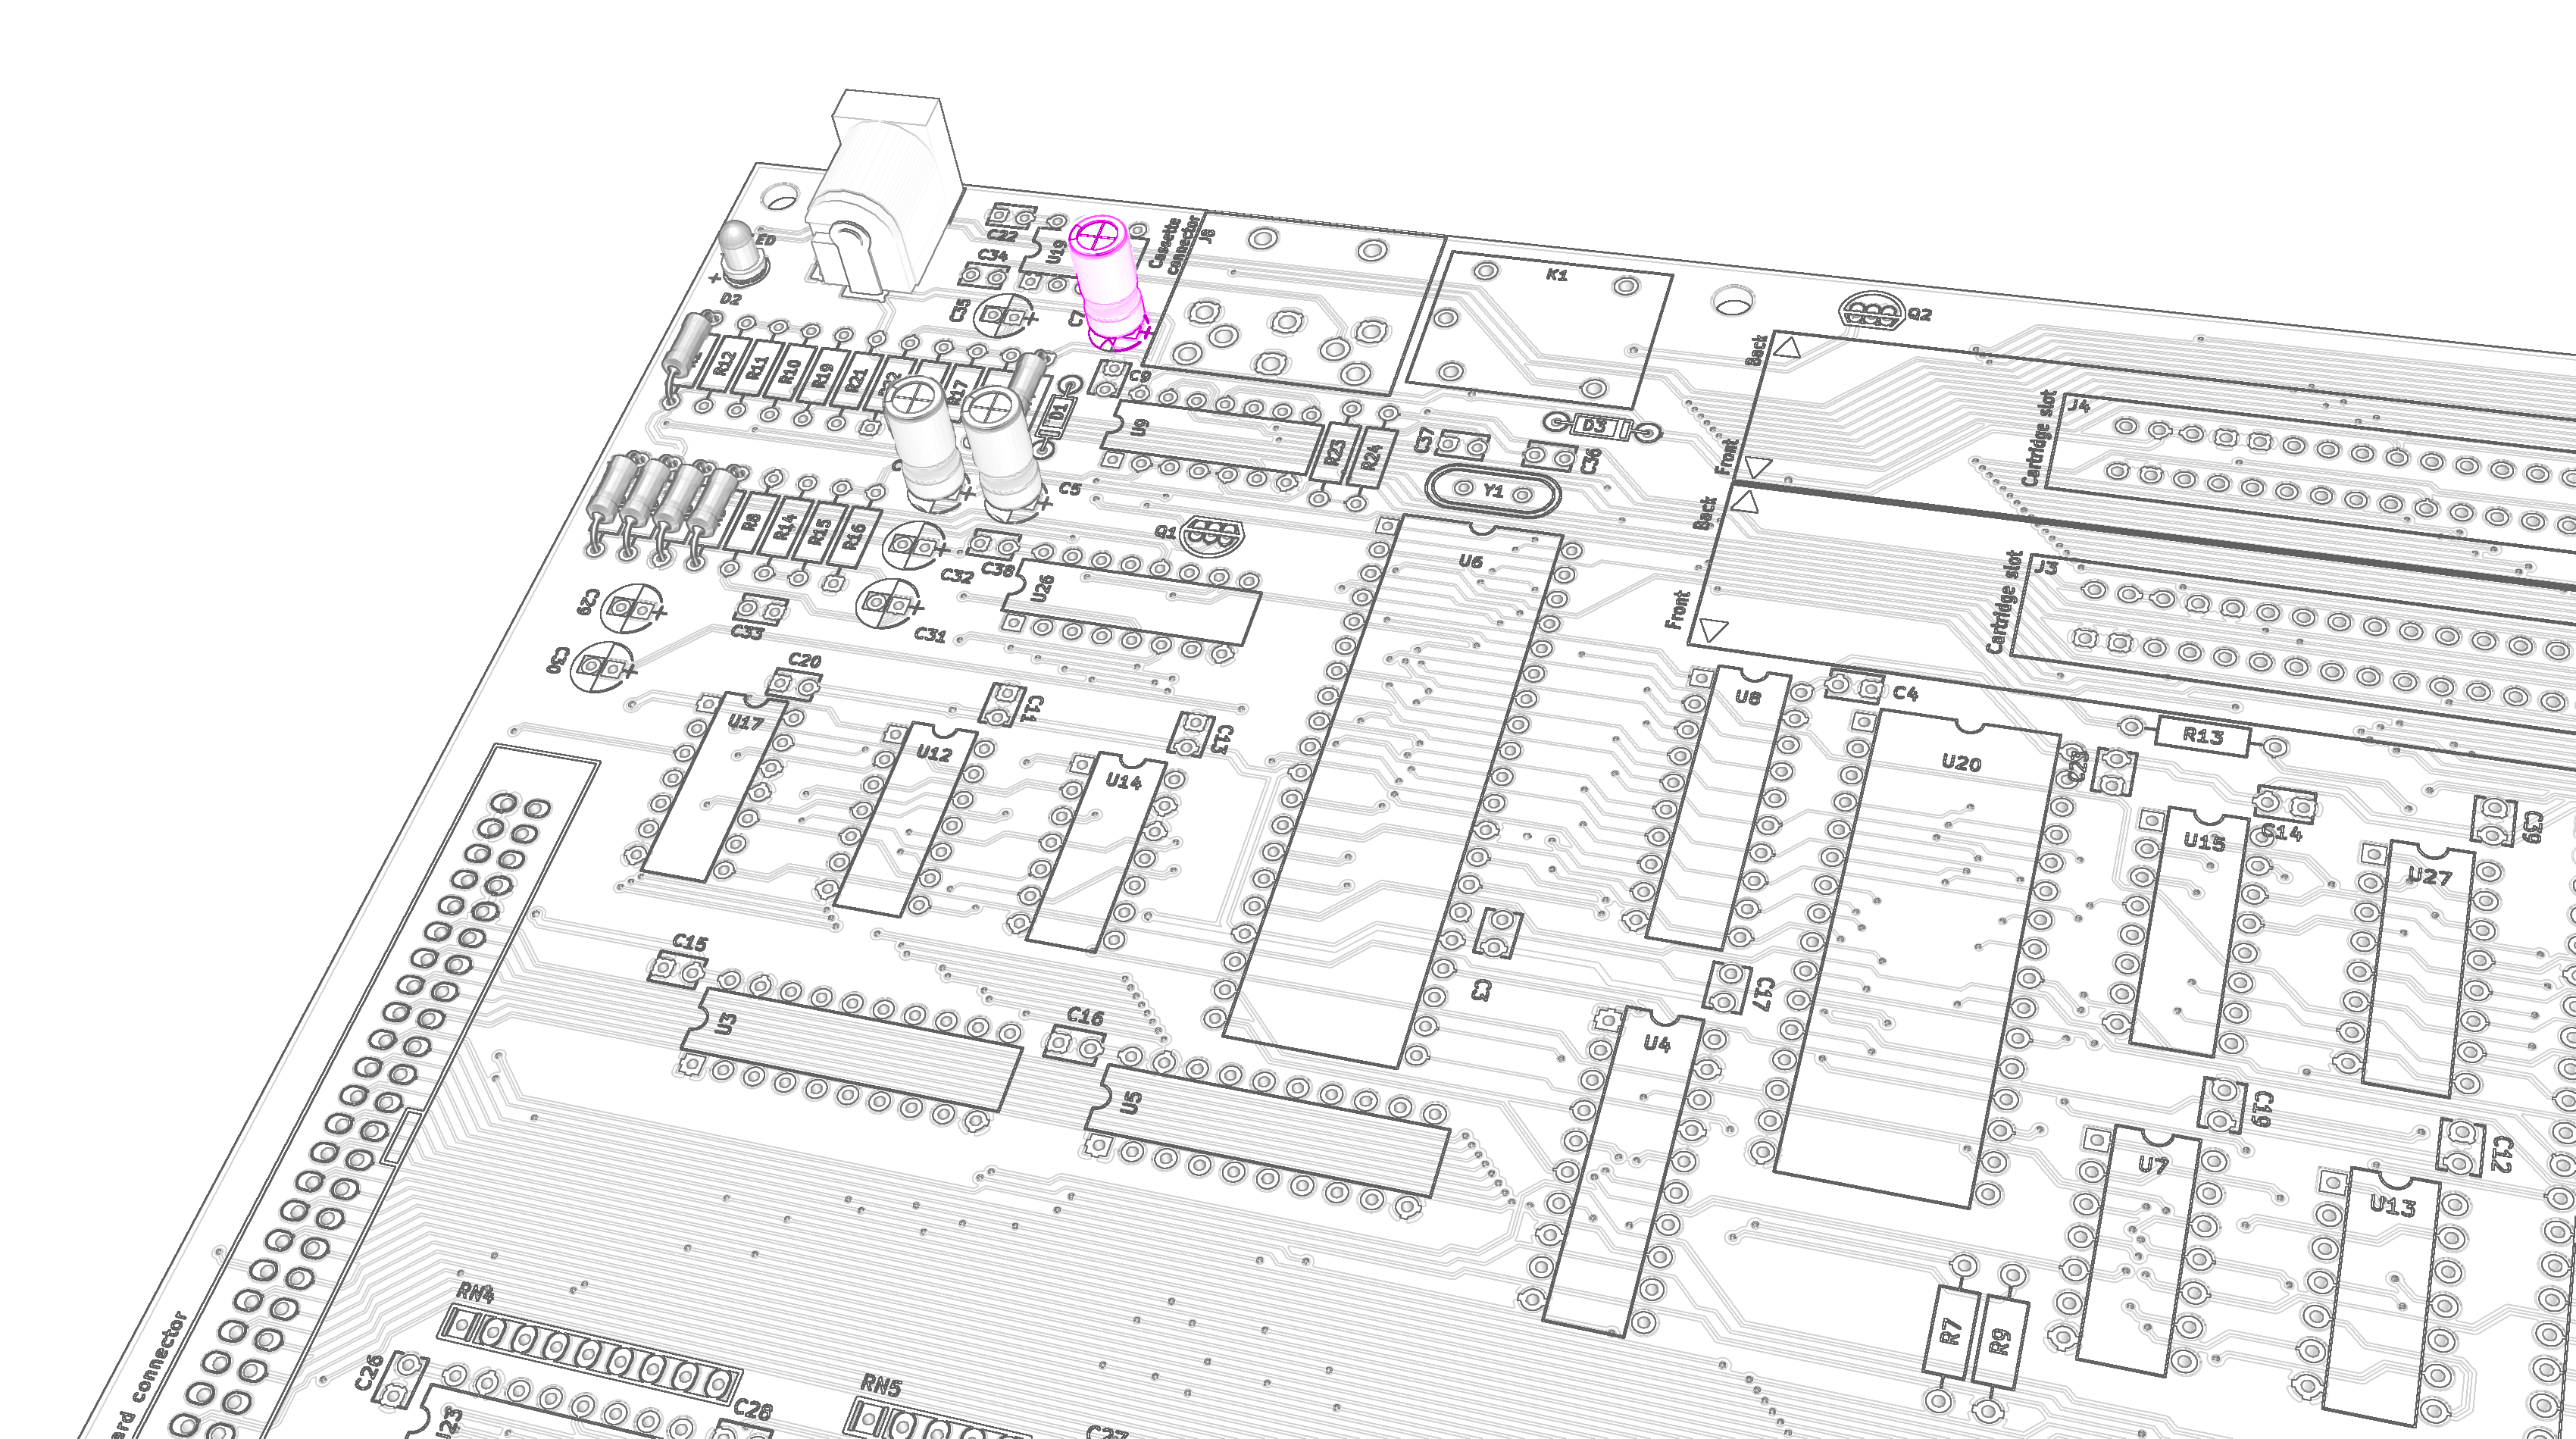
\includegraphics[width=0.8\linewidth]{figures/mount-power-05}
  \caption{Placement of capacitor {\tt C7}}
  \label{fig:mount-power-05}
\end{figure}

\begin{figure}[htbp]
  \centering
  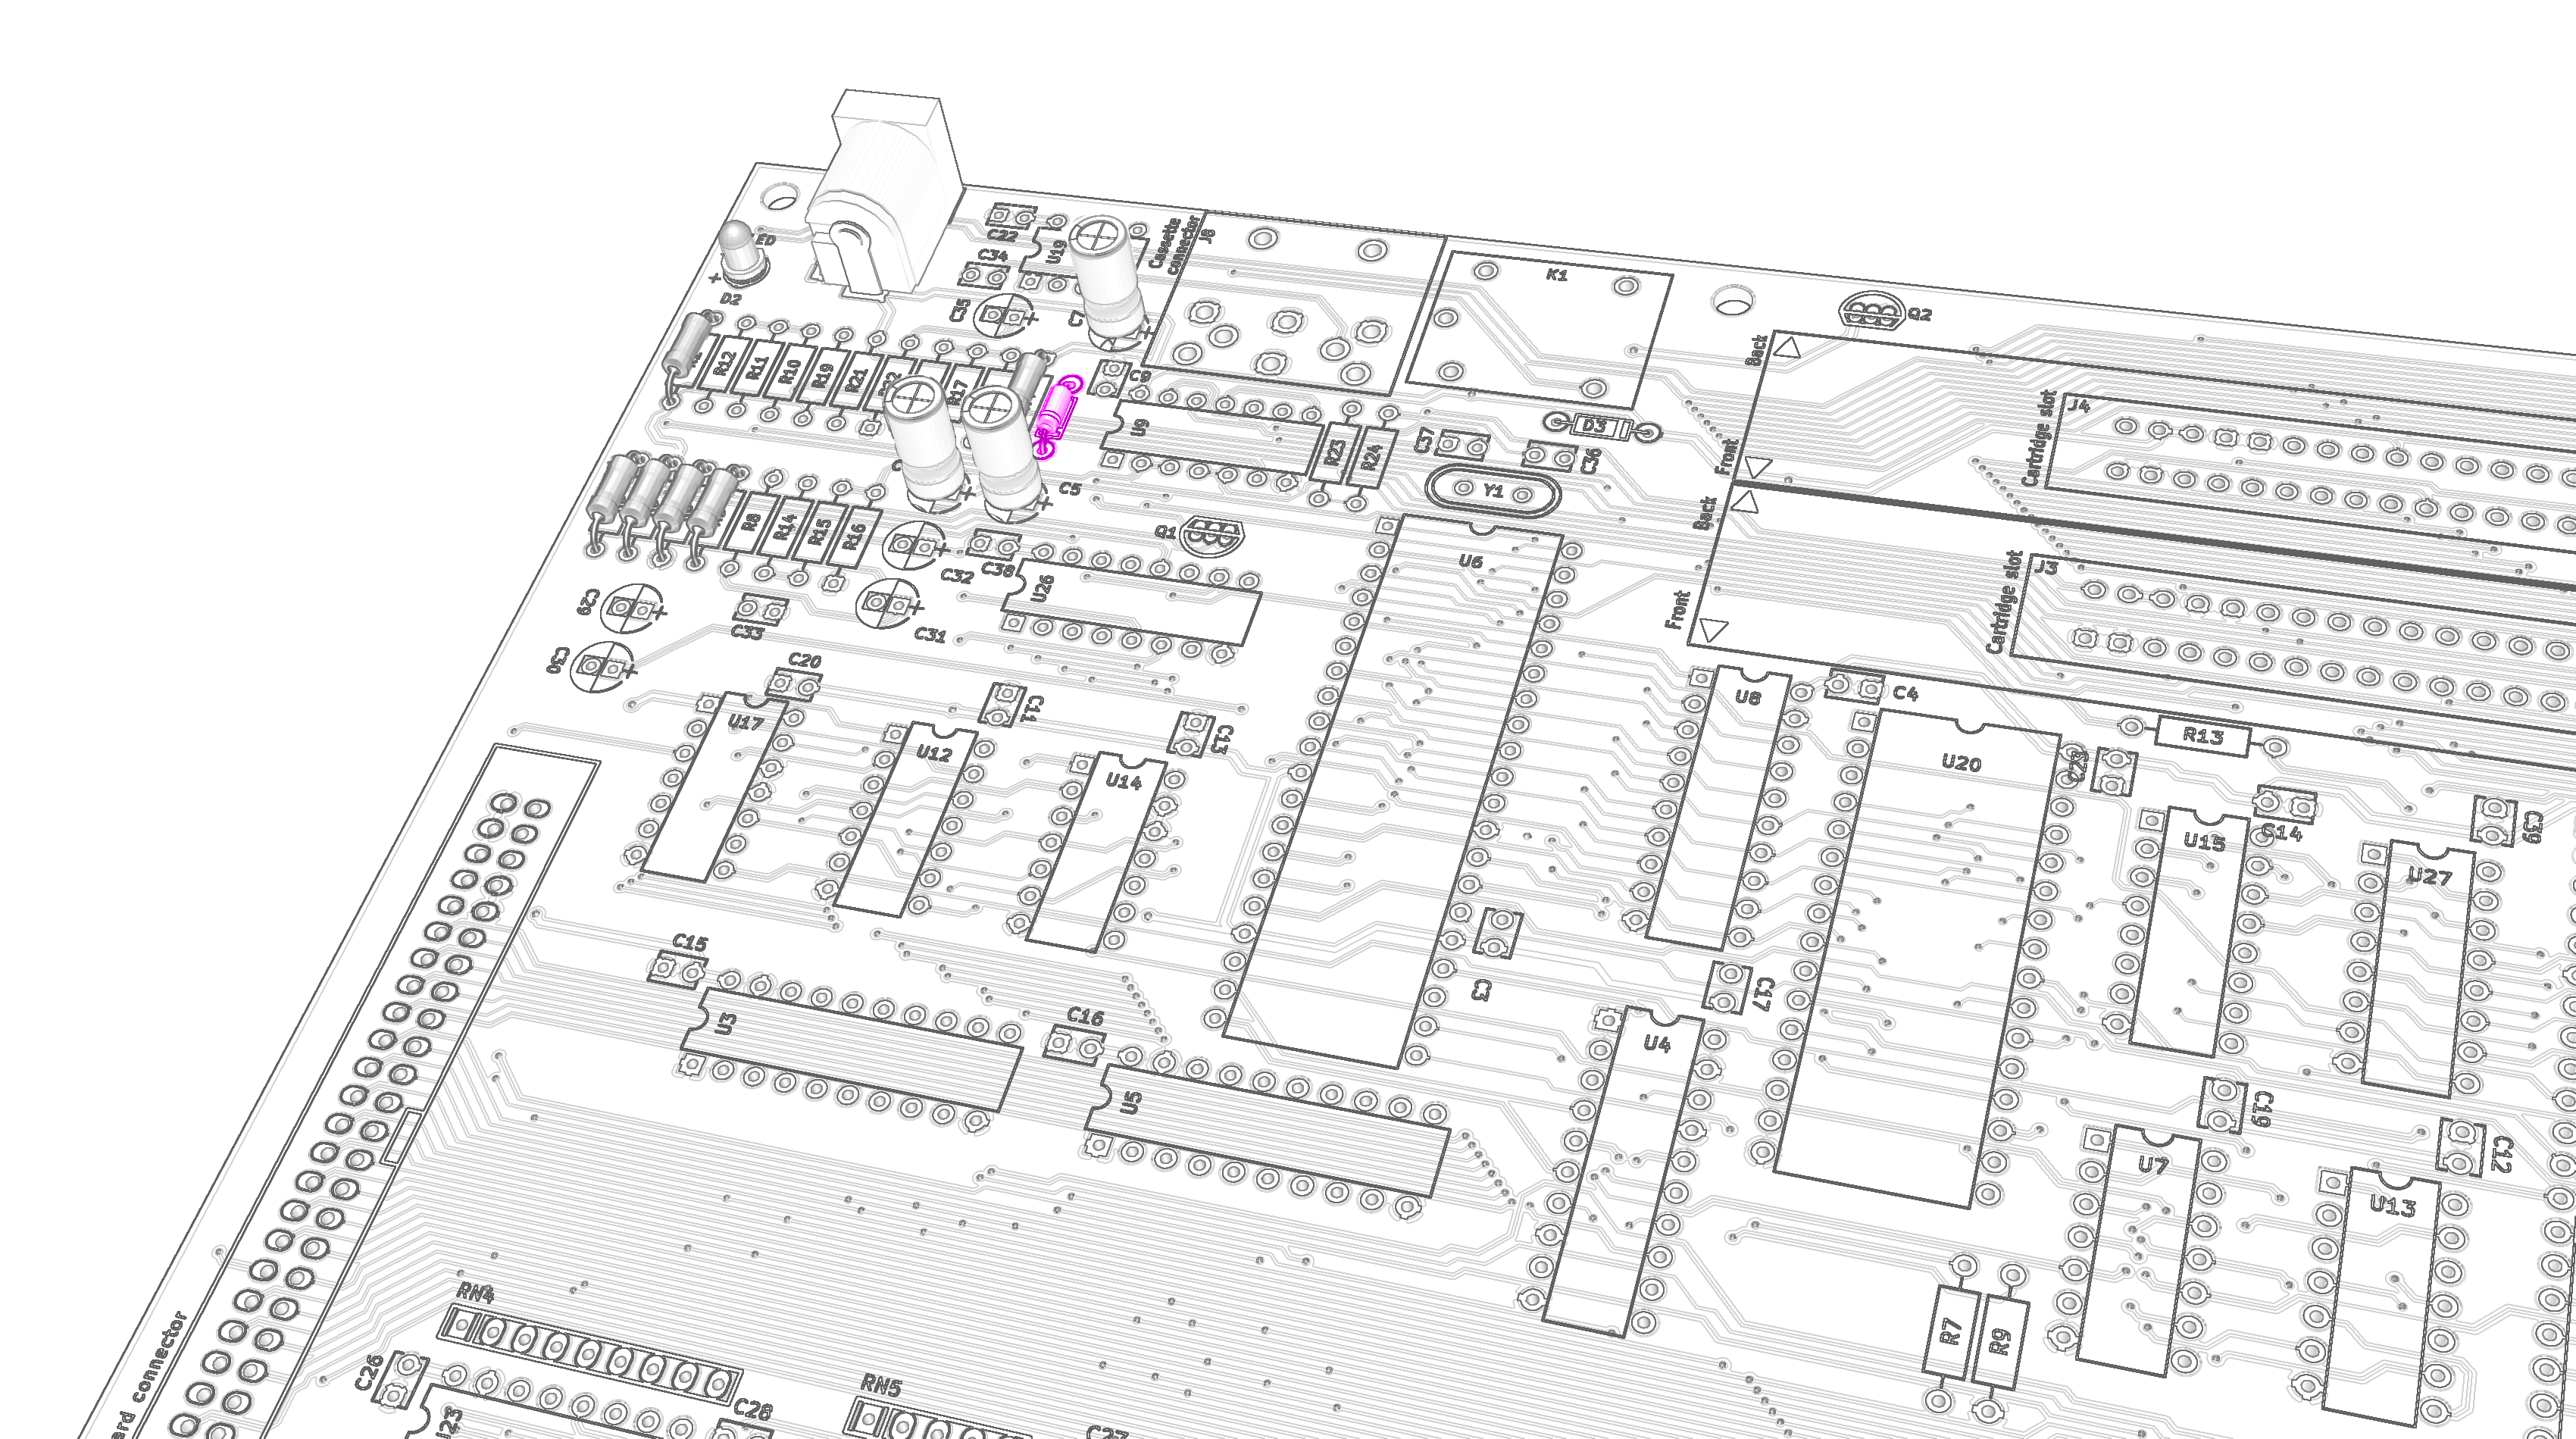
\includegraphics[width=0.8\linewidth]{figures/mount-power-06}
  \caption{Placement of diode {\tt D1}}
  \label{fig:mount-power-06}
\end{figure}

\begin{figure}[htbp]
  \centering
  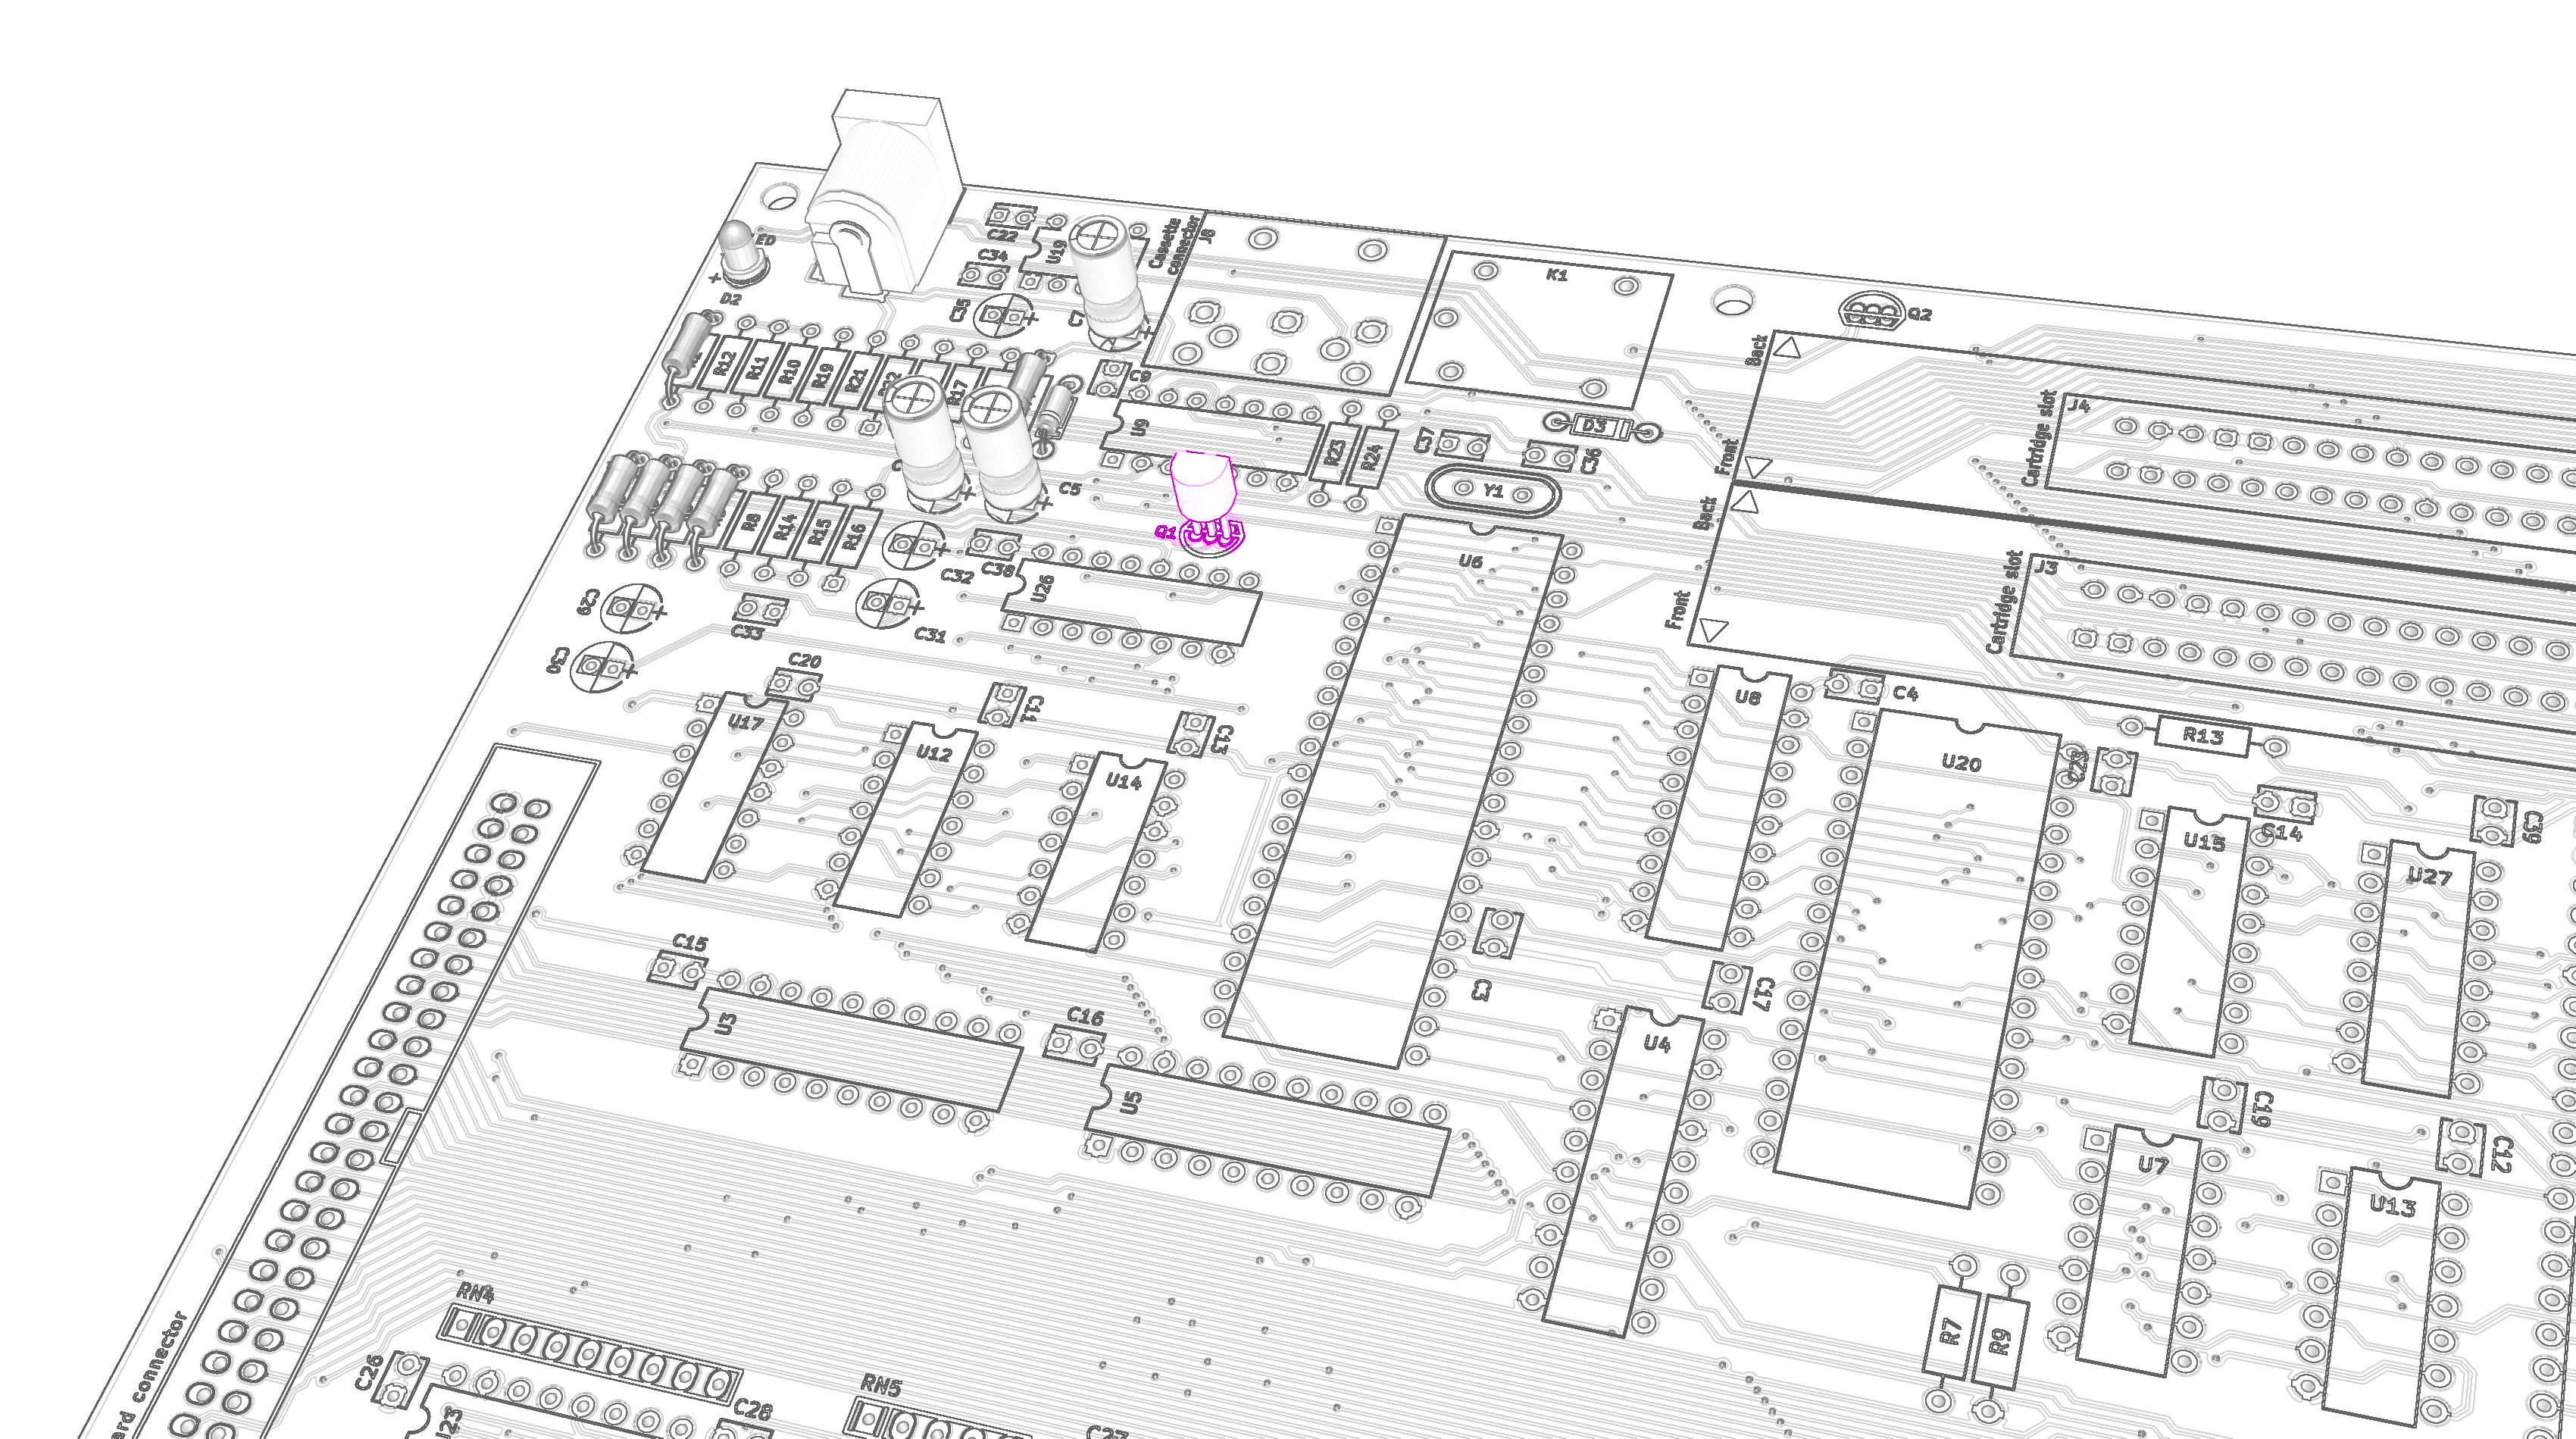
\includegraphics[width=0.8\linewidth]{figures/mount-power-07}
  \caption{Placement of transistor {\tt Q1}}
  \label{fig:mount-power-07}
\end{figure}

\begin{figure}[htbp]
  \centering
  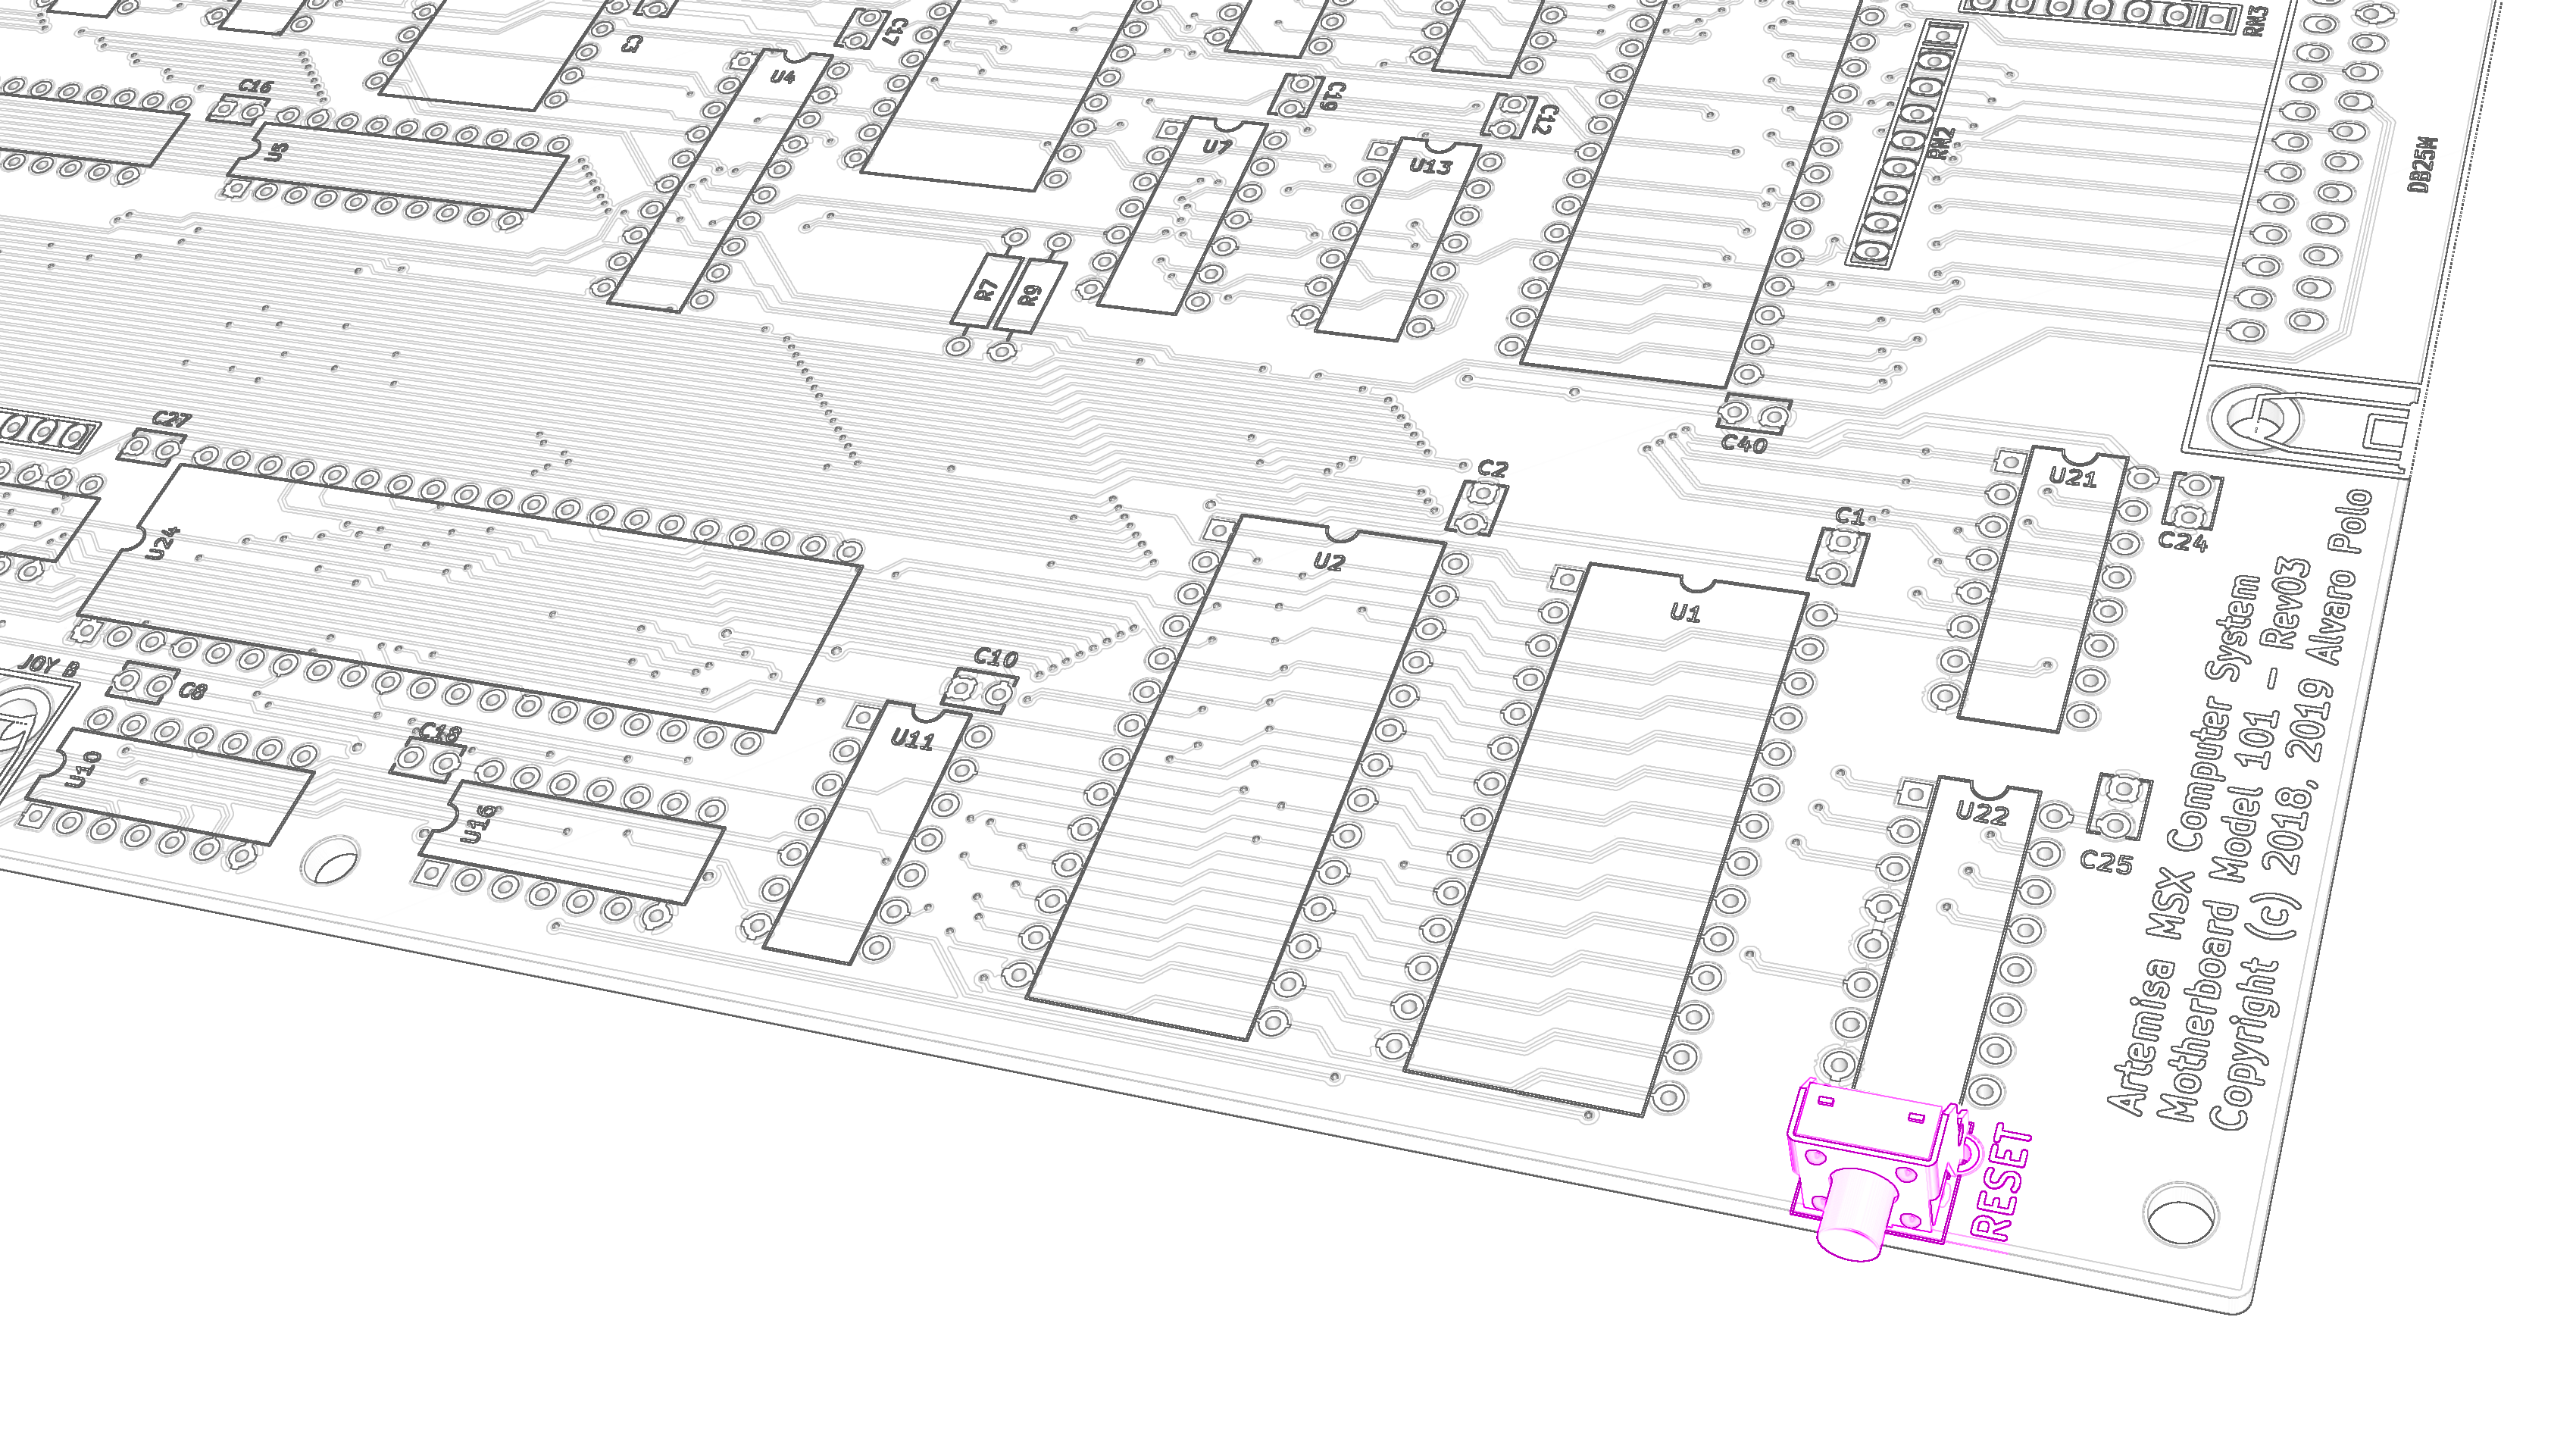
\includegraphics[width=0.8\linewidth]{figures/mount-power-08}
  \caption{Placement of push button {\tt SW1}}
  \label{fig:mount-power-08}
\end{figure}

\begin{figure}[htbp]
  \centering
  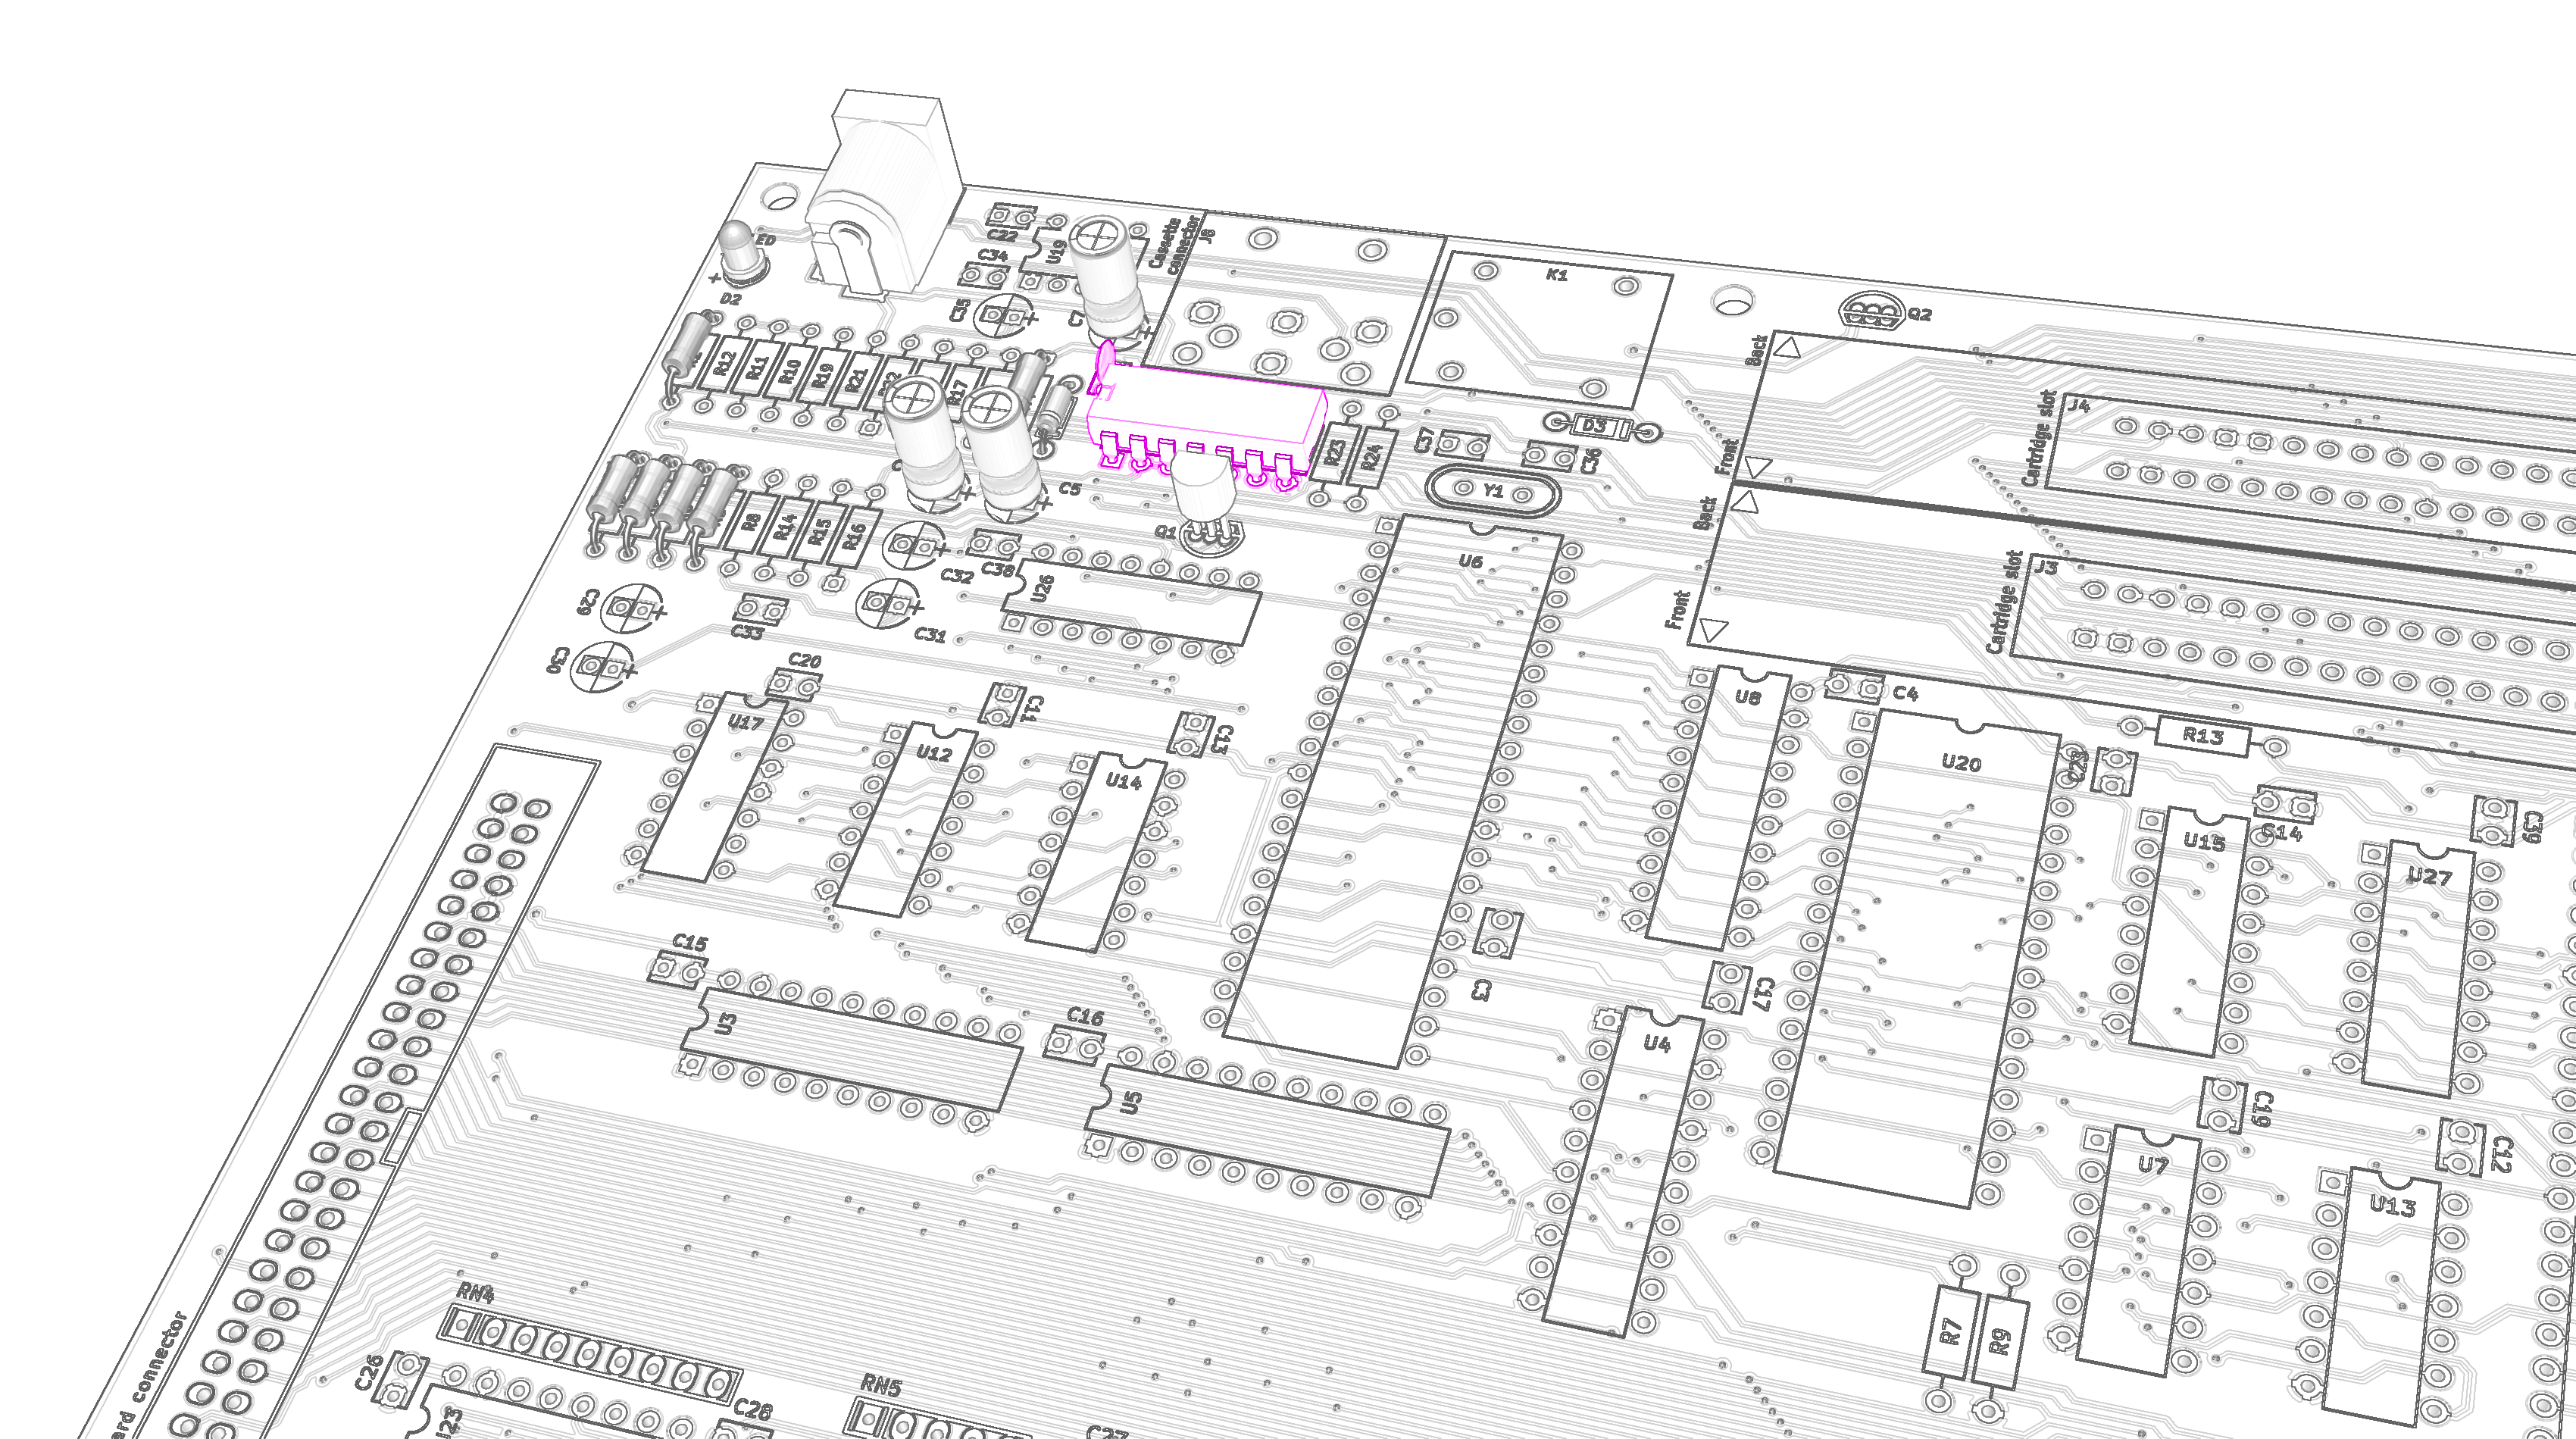
\includegraphics[width=0.8\linewidth]{figures/mount-power-09}
  \caption{Placement of IC {\tt U9} and its decoupling capacitor {\tt C9}}
  \label{fig:mount-power-09}
\end{figure}

Once all these parts are assembled, we can make a few tests to see if everything working fine. If you have an oscilloscope or a logic analyzer, you can follow these steps:

\begin{enumerate}
  \item Connect a probe with the positive terminal to {\tt /RESET} at the pin 6 of {\tt UC9} and the negative terminal to {\tt GND} at pin 7 of {\tt U9}.
  \item Connect another probe with the positive terminal to {\tt 5+} at the pin 14 of {\tt UC9} and the negative terminal to {\tt GND} at pin 7 of {\tt U9}.
  \item Configure the second probe connected to {\tt 5+} as a rising edge trigger so we can capture data once the power is connected.
  \item Plug the power adapter cable into the DC barrel connector.
  \item Your oscilloscope or logic analyzer will capture the {\tt 5+} and {\tt /RESET} signals. The {\tt /RESET} signal will stabilize to low once {\tt 5+} stabilizes to 5v. You have to see a low reset pulse from 100ms to 150ms length.
  \item Prepare the oscilloscope or logic analyzer for a new capture. This time using the first probe connected to {\tt /RESET} as a falling edge trigger.
  \item Press the reset button {\tt SW1}.
  \item Your oscilloscope or logic analyzer will capture a new reset pulse. This time it might be longer than before, as it depends on how much time you kept pushing the reset button.
\end{enumerate}

If you just have a multimeter, you can test the circuit as follows:

\begin{enumerate}
  \item Connect the probe with the positive terminal to {\tt /RESET} at the pin 6 of {\tt UC9} and the negative terminal to {\tt GND} at pin 7 of {\tt U9}.
  \item Configure the multimeter to measure DC voltage.
  \item Plug the power adapter cable into the DC barrel connector.
  \item Your multimeter have to show a value close to 5 volts.
  \item Press the reset button {\tt SW1} and keep it pressed.
  \item Your multimeter have to show a value of 0 volts.
  \item Release the reset button {\tt SW1}.
  \item Your multimeter have to show again a value close to 5 volts.
\end{enumerate}

If you do not have an oscilloscope, a logic analyzer or a multipleter at hand, there is nothing to be tested here.

